\documentclass[../thesis.tex]{subfiles}
\begin{document}

\chapter{Lines profiles}
\label{cap:appendix1}

\section{IC 5063}

\begin{figure*}
\centering
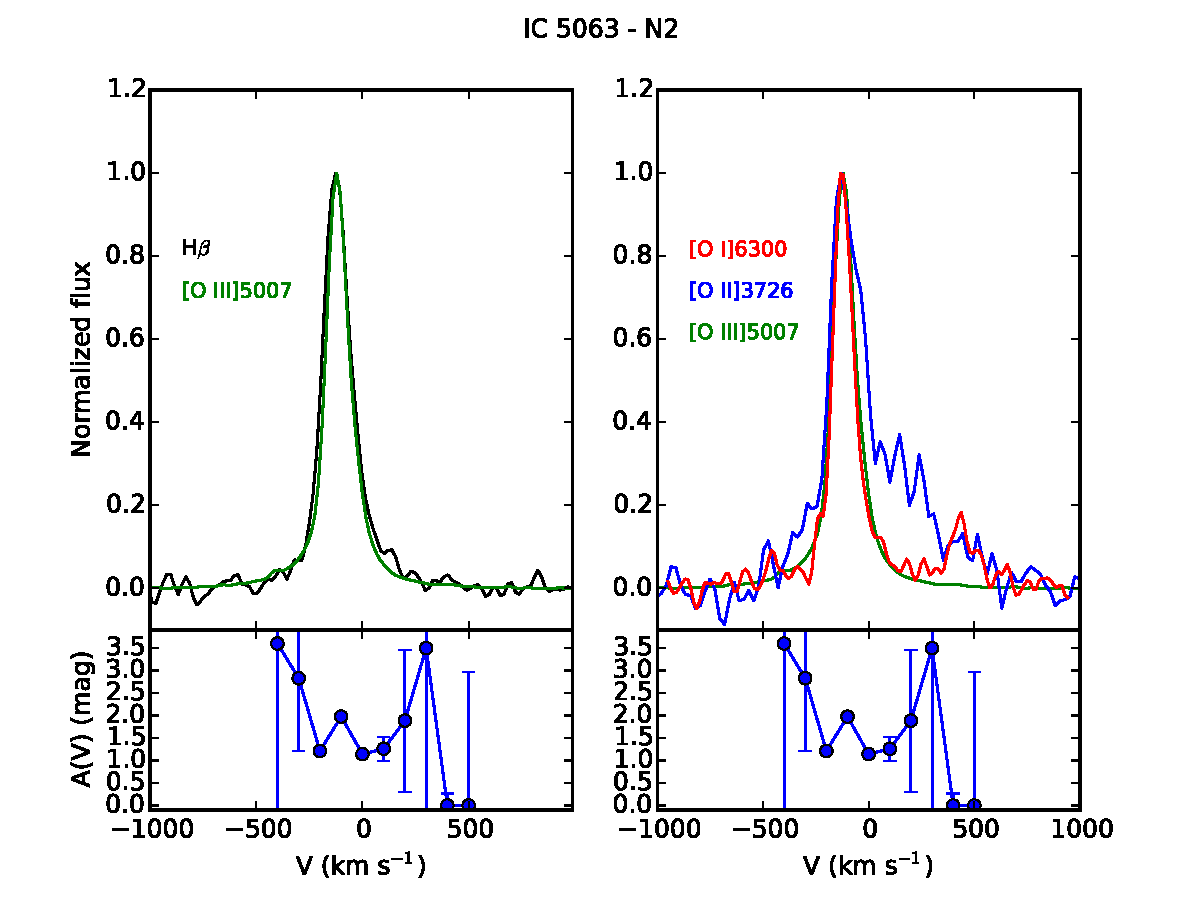
\includegraphics[width=0.45\textwidth]{images/paper1/IC5063_n2_l1.pdf} \quad
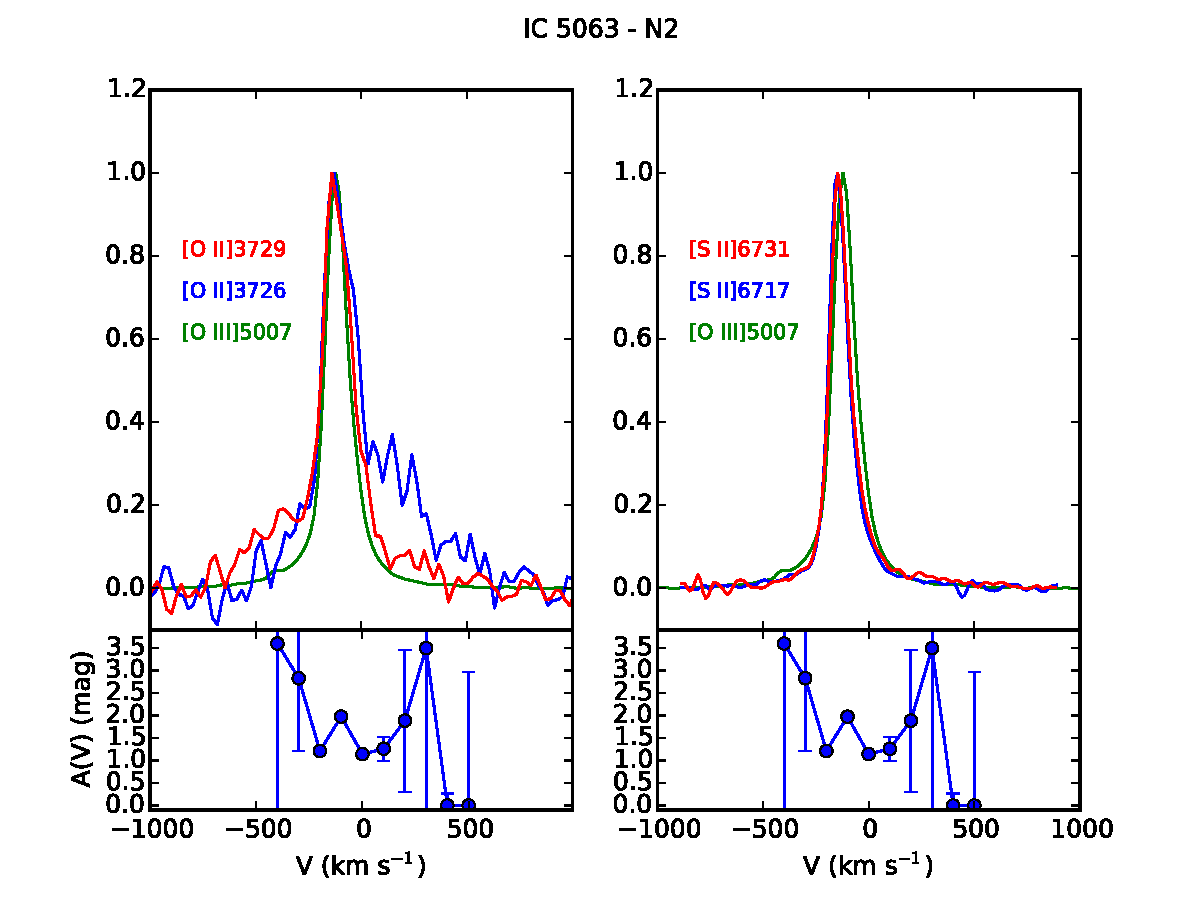
\includegraphics[width=0.45\textwidth]{images/paper1/IC5063_n2_l2.pdf}\\
\caption[]{Comparison of the emission lines of the N2 region of IC\,5063. The behaviour of the extinction coefficient as a function of velocity is shown under each plot.}
\label{fig:n2l1_I}
\end{figure*}

\begin{figure*}
\centering
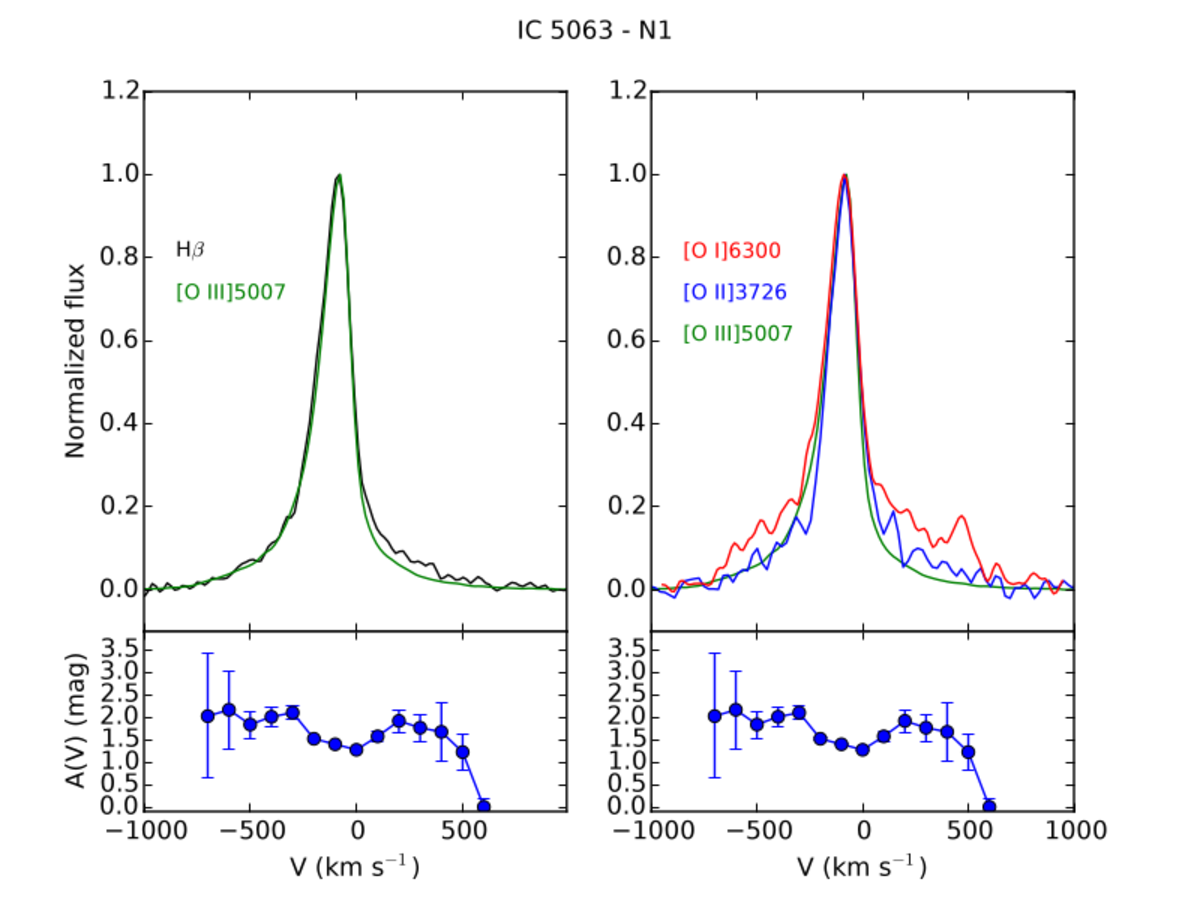
\includegraphics[width=0.45\textwidth]{images/paper1/IC5063_n1_l1.pdf} \quad
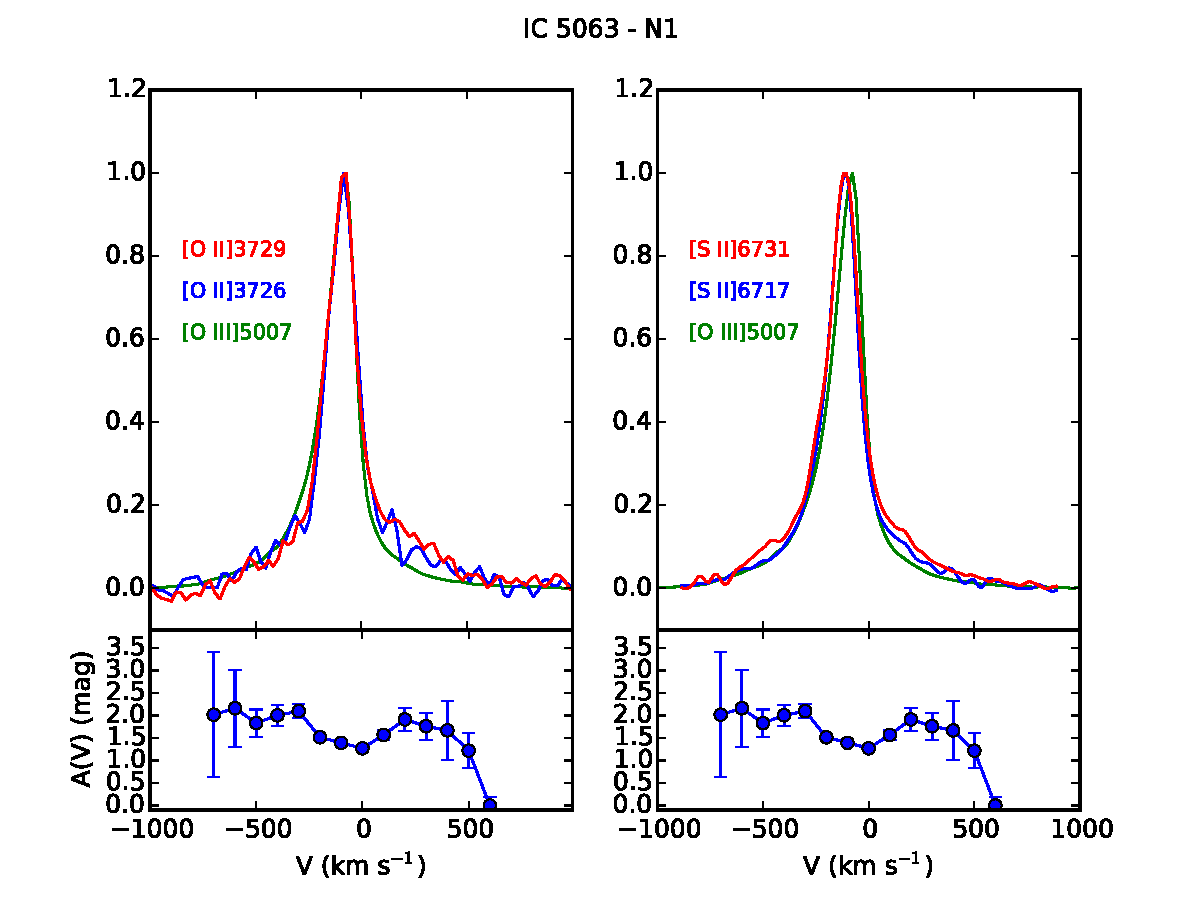
\includegraphics[width=0.45\textwidth]{images/paper1/IC5063_n1_l2.pdf}\\
\caption[]{Comparison of the emission lines of the N1 region of IC\,5063. The behaviour of the extinction coefficient as a function of velocity is shown under each plot.}
\label{fig:n1l1_I}
\end{figure*}


\begin{figure*}
\centering
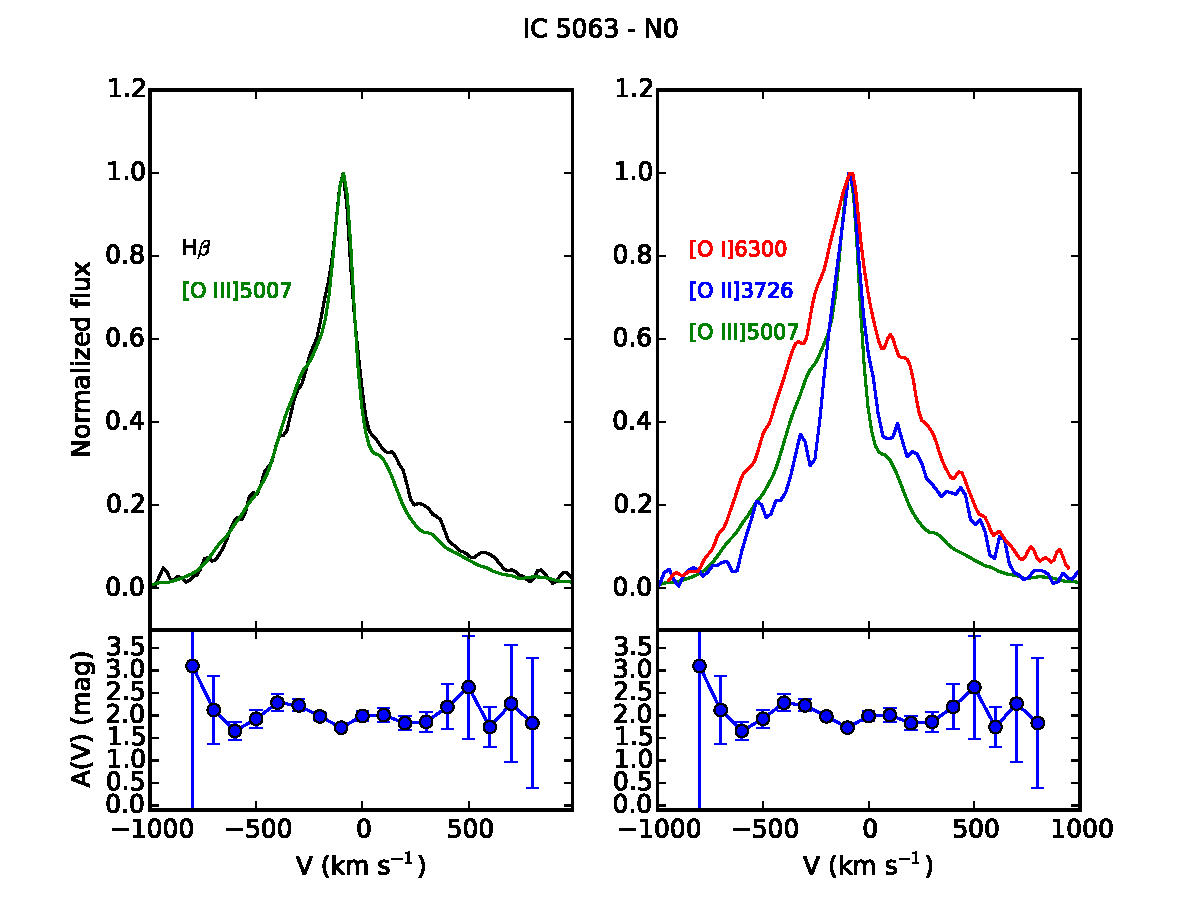
\includegraphics[width=0.45\textwidth]{images/paper1/IC5063_n0_l1.pdf} \quad
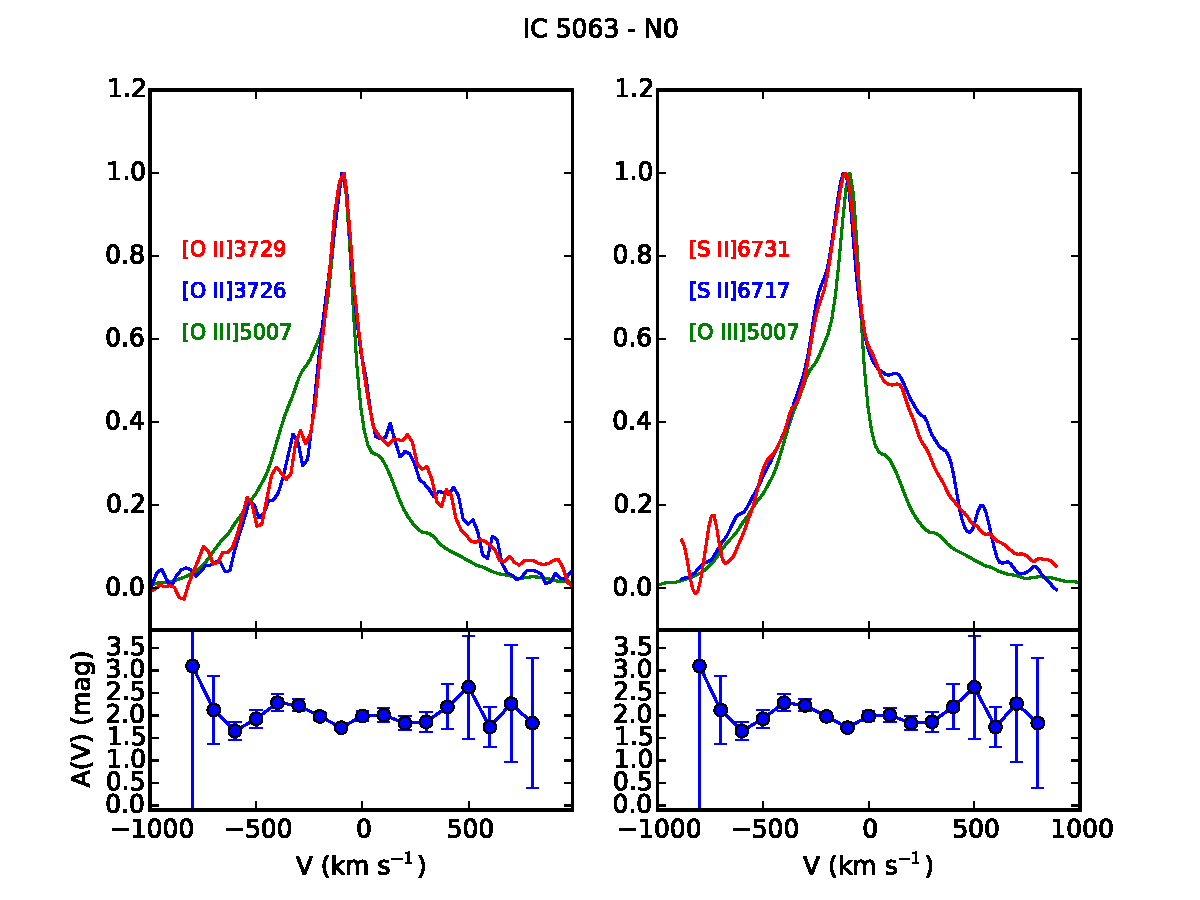
\includegraphics[width=0.45\textwidth]{images/paper1/IC5063_n0_l2.pdf}\\
\caption[]{Comparison of the emission lines of the N0 region of IC\,5063. The behaviour of the extinction coefficient as a function of velocity is shown under each plot.}
\label{fig:n0l1_I}
\end{figure*}

\begin{figure*}
\centering
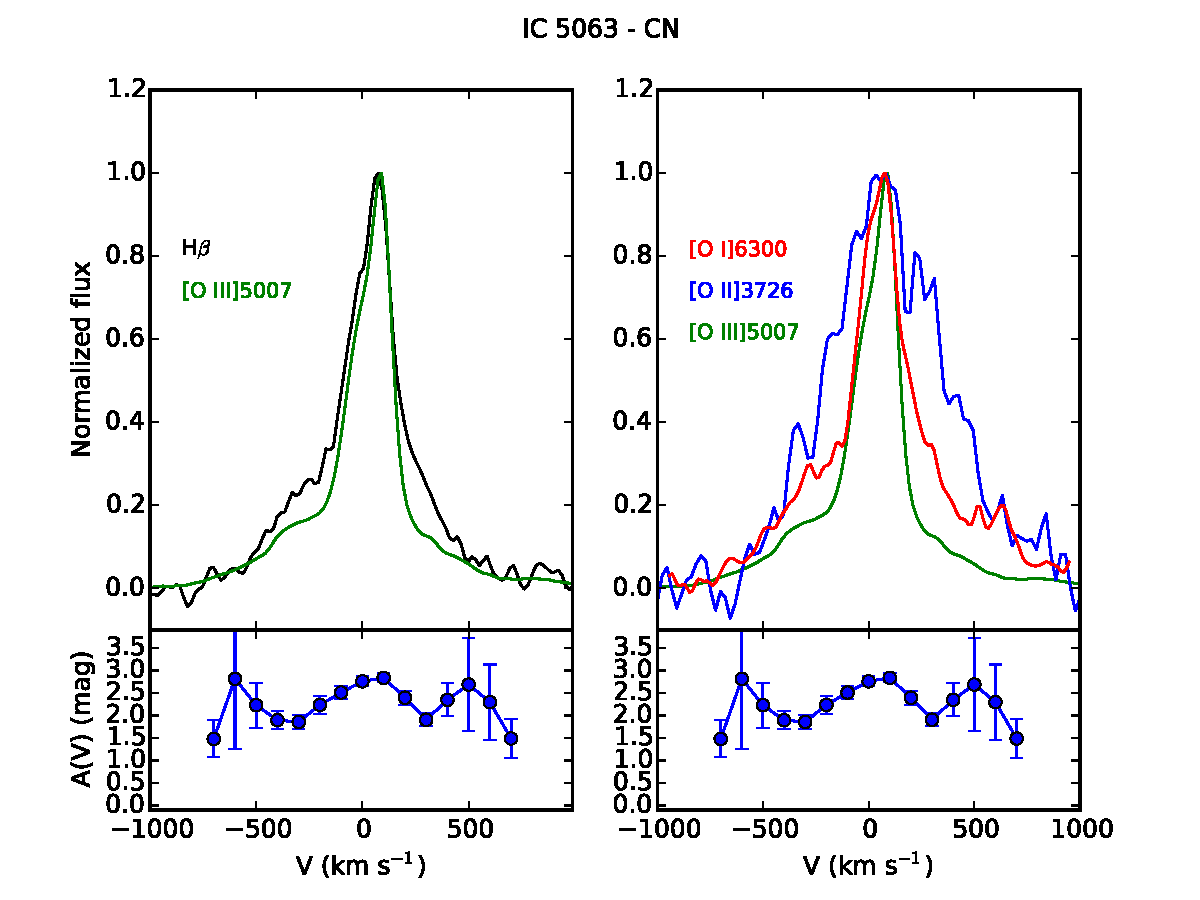
\includegraphics[width=0.45\textwidth]{images/paper1/IC5063_cn_l1.pdf} \quad
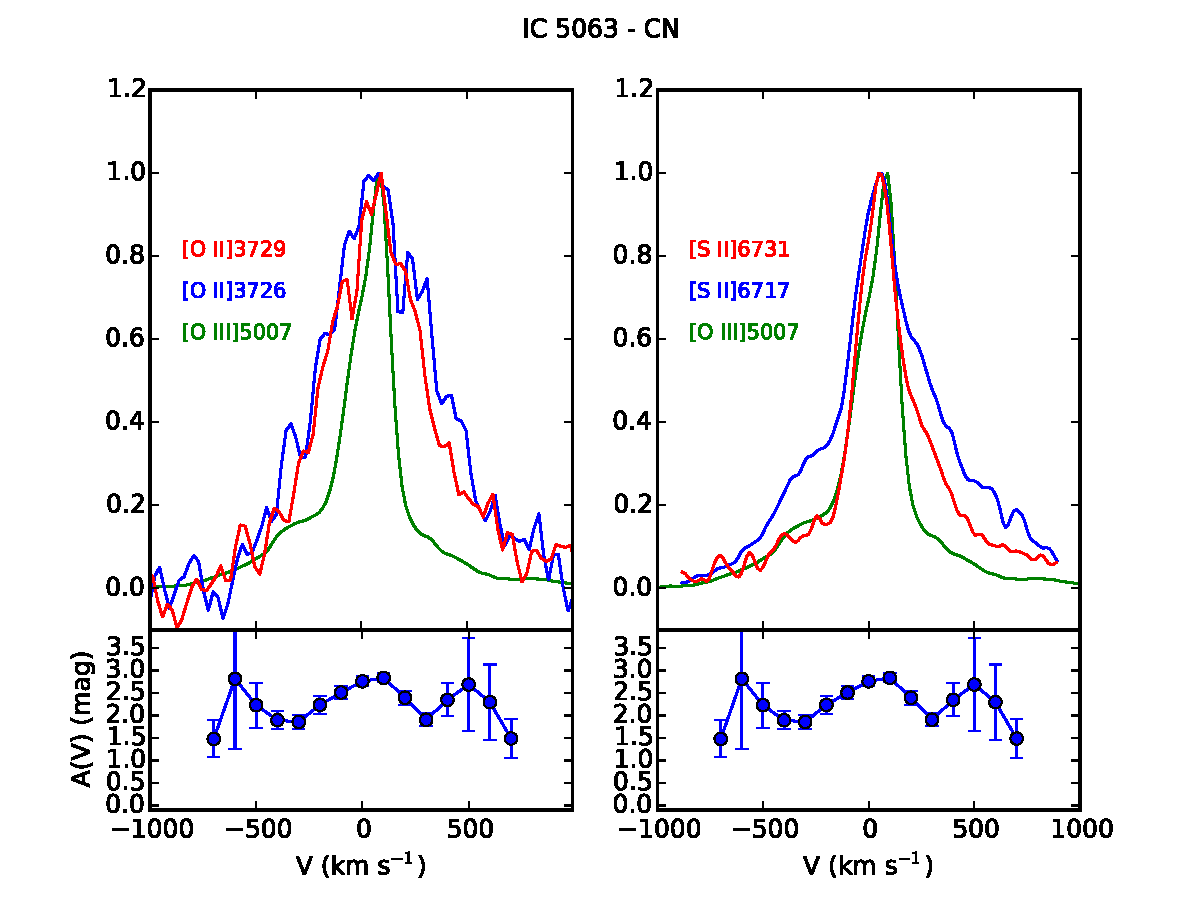
\includegraphics[width=0.45\textwidth]{images/paper1/IC5063_cn_l2.pdf}\\
\caption[]{Comparison of the emission lines of the CN region of IC\,5063. The behaviour of the extinction coefficient as a function of velocity is shown under each plot.}
\label{fig:cnl1_I}
\end{figure*}

\begin{figure*}
\centering
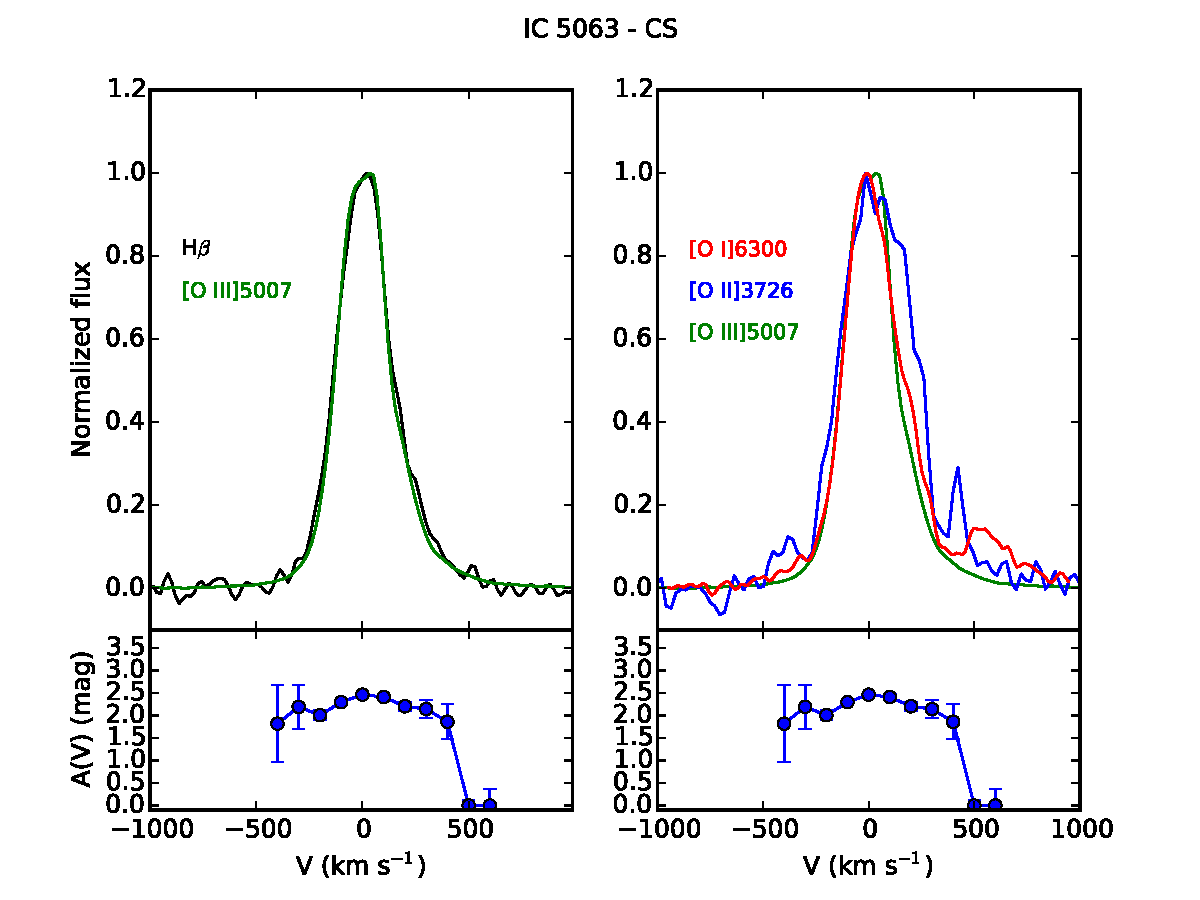
\includegraphics[width=0.45\textwidth]{images/paper1/IC5063_cs_l1.pdf} \quad
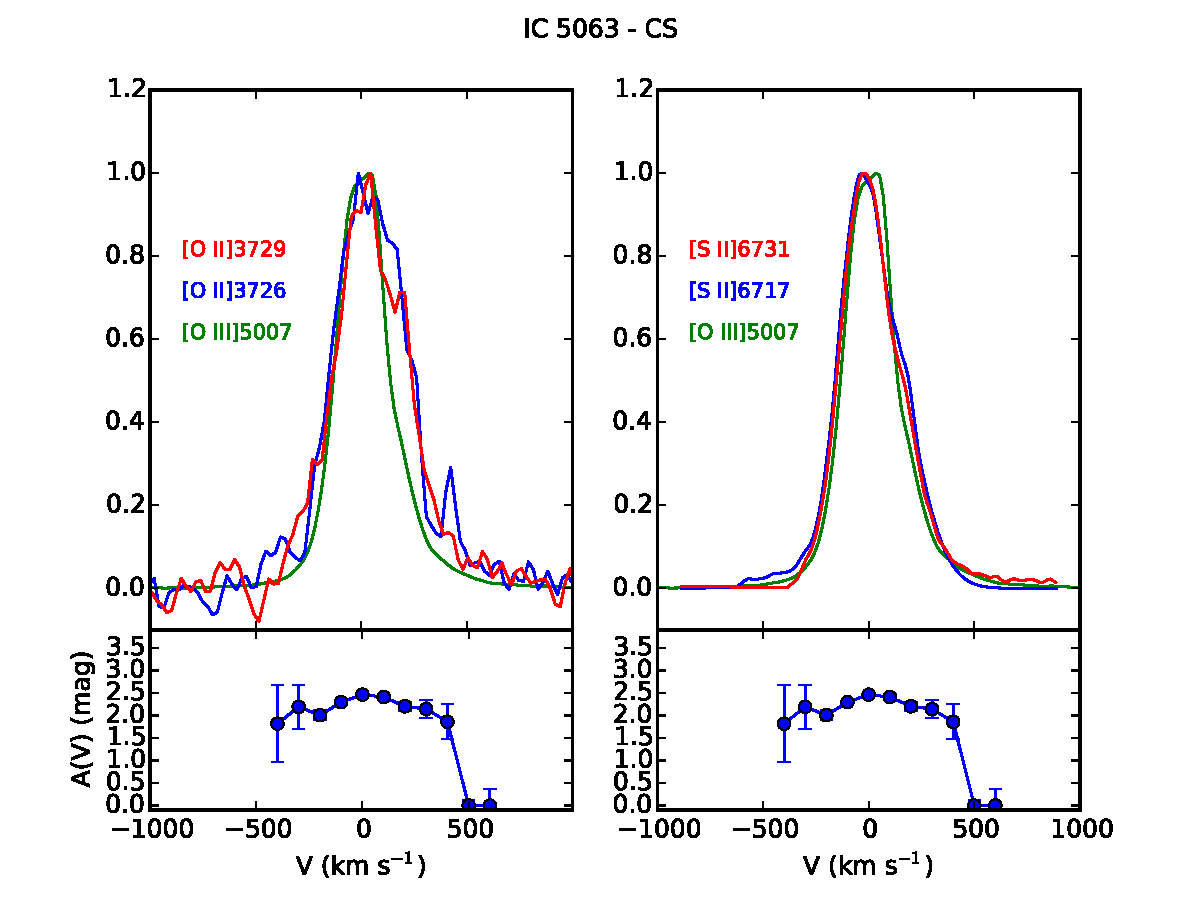
\includegraphics[width=0.45\textwidth]{images/paper1/IC5063_cs_l2.pdf}\\
\caption[]{Comparison of the emission lines of the CS region of IC\,5063. The behaviour of the extinction coefficient as a function of velocity is shown under each plot.}
\label{fig:csl1_I}
\end{figure*}

\begin{figure*}
\centering
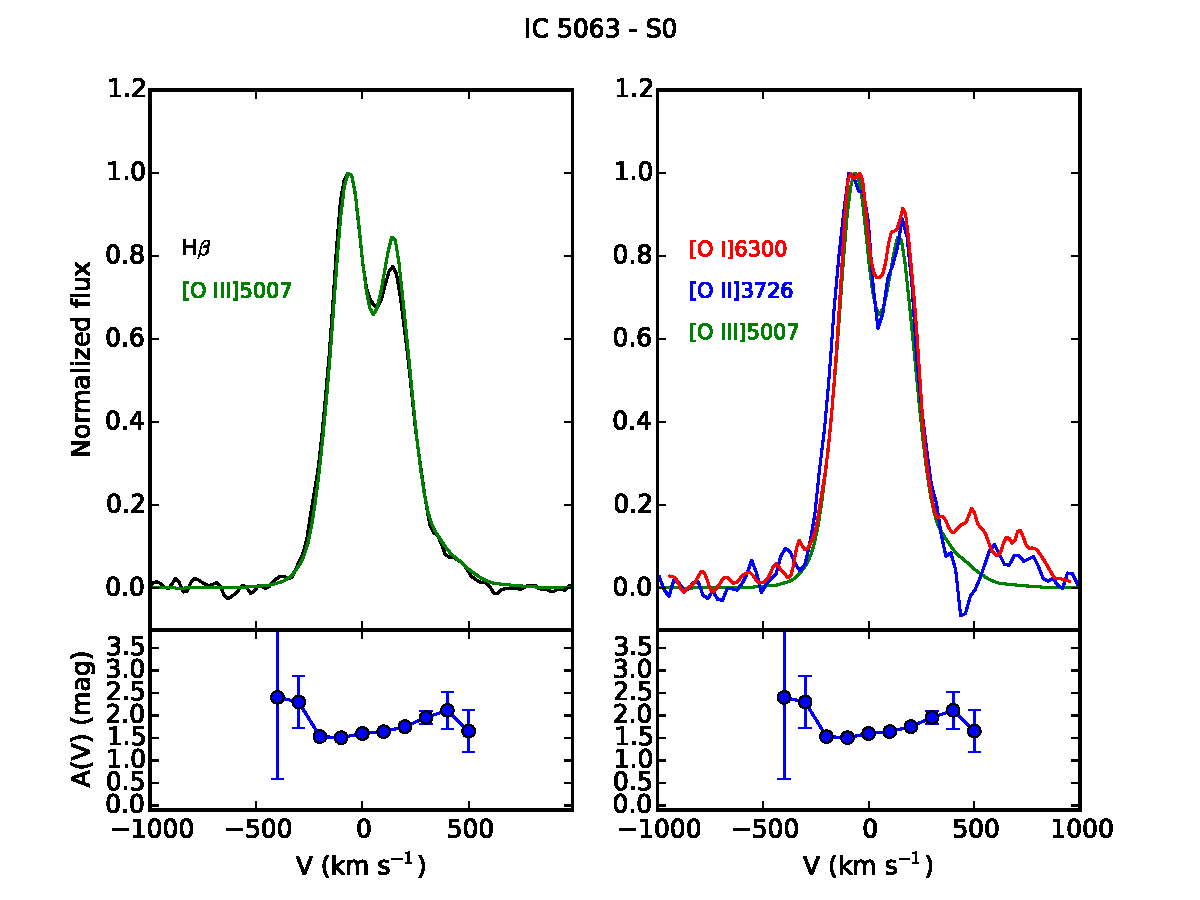
\includegraphics[width=0.45\textwidth]{images/paper1/IC5063_s0_l1.pdf} \quad
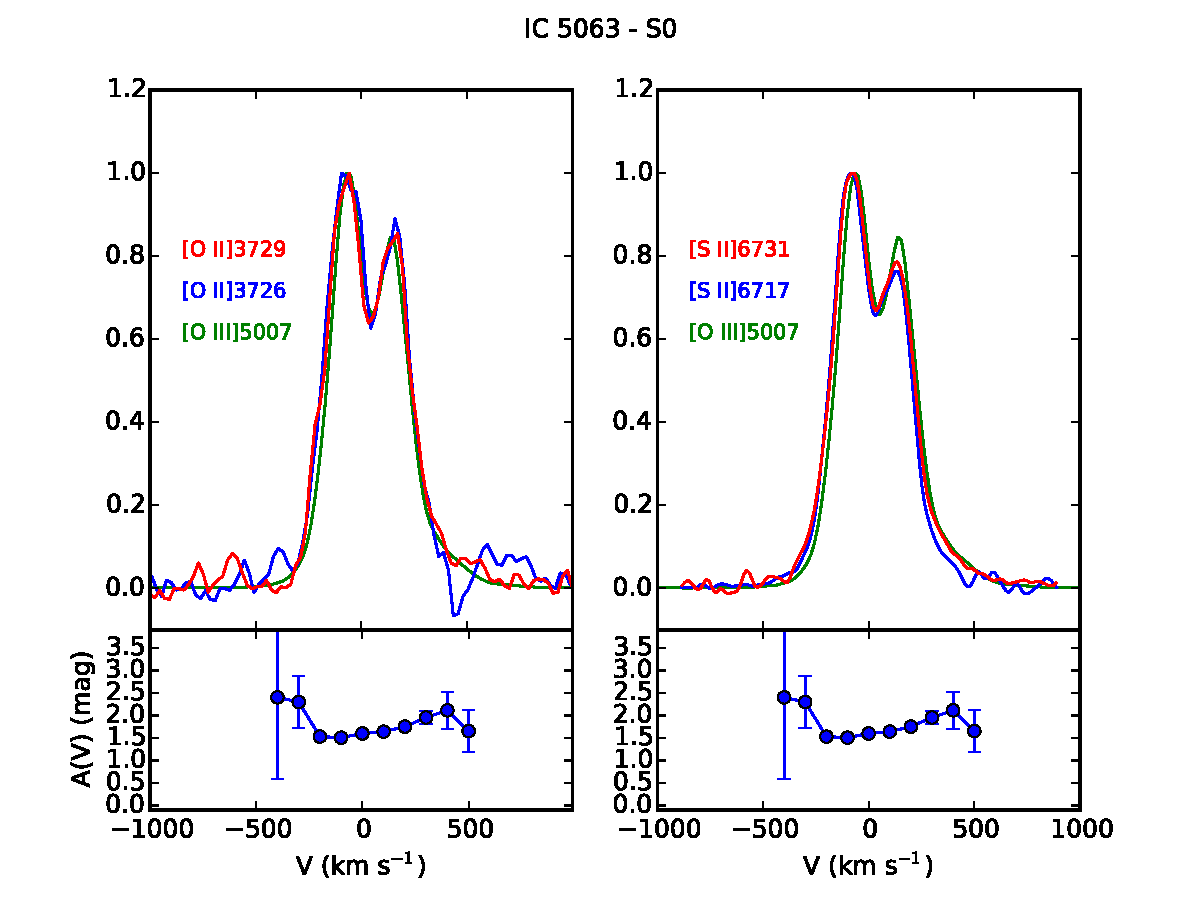
\includegraphics[width=0.45\textwidth]{images/paper1/IC5063_s0_l2.pdf}\\
\caption[]{Comparison of the emission lines of the S0 region of IC\,5063. The behaviour of the extinction coefficient as a function of velocity is shown under each plot.}
\label{fig:s0l1_I}
\end{figure*}

\begin{figure*}
\centering
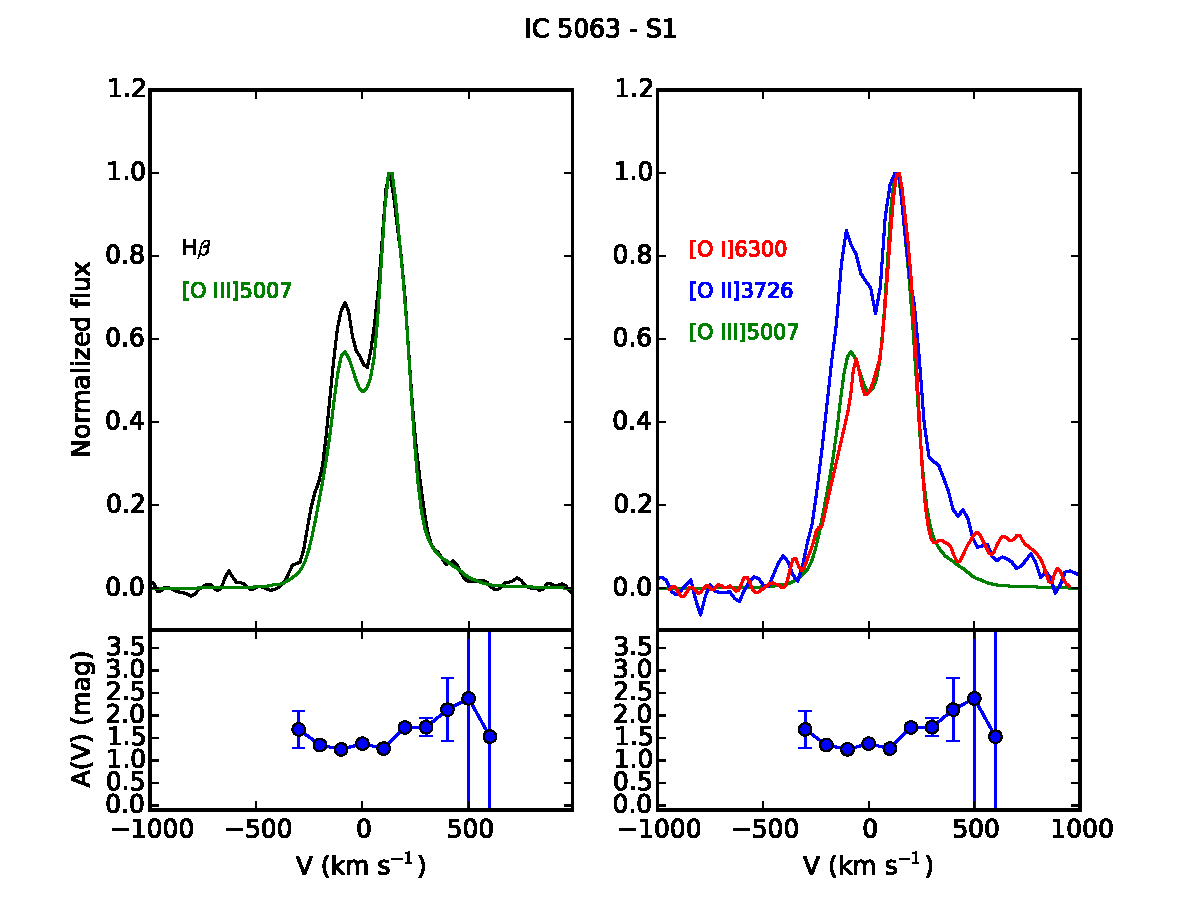
\includegraphics[width=0.45\textwidth]{images/paper1/IC5063_s1_l1.pdf} \quad
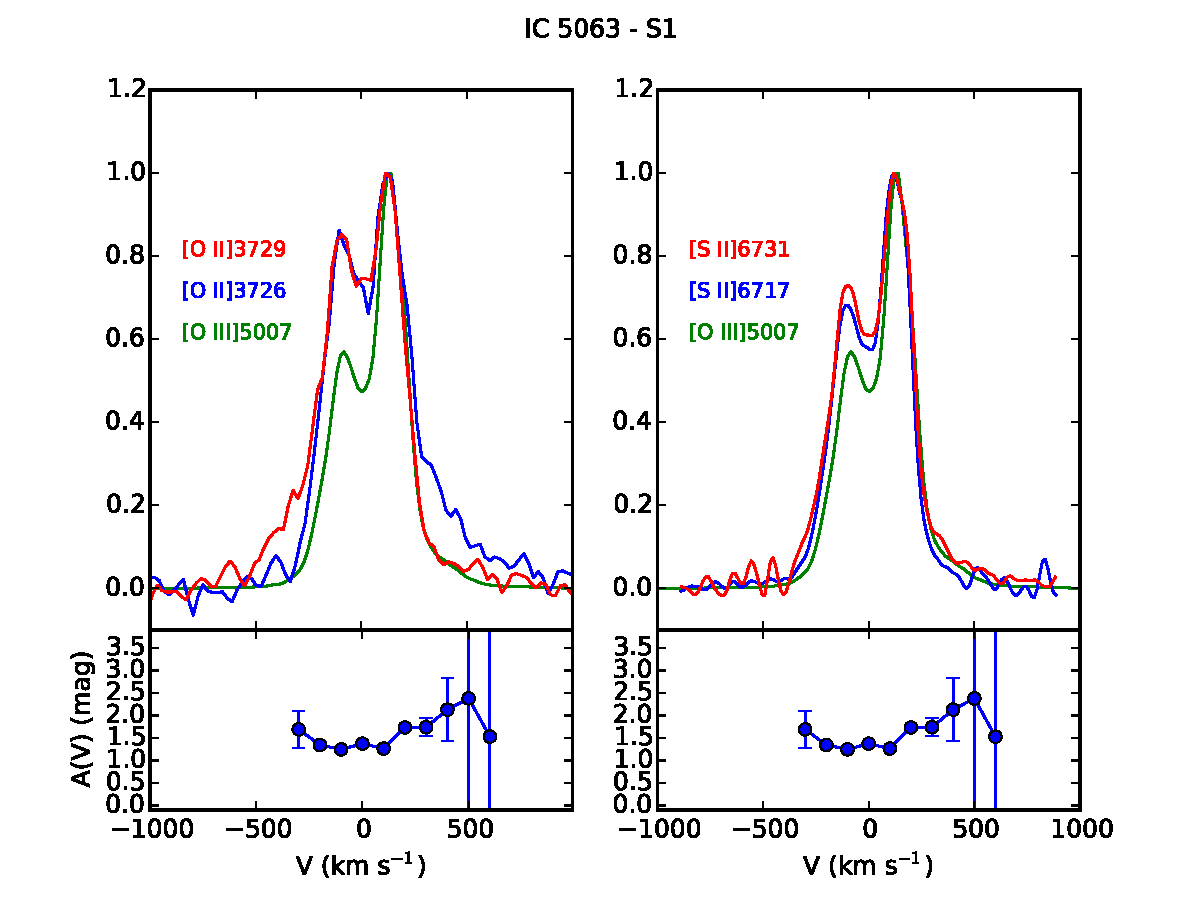
\includegraphics[width=0.45\textwidth]{images/paper1/IC5063_s1_l2.pdf}\\
\caption[]{Comparison of the emission lines of the S1 region of IC\,5063. The behaviour of the extinction coefficient as a function of velocity is shown under each plot.}
\label{fig:s1l1_I}
\end{figure*}

\begin{figure*}
\centering
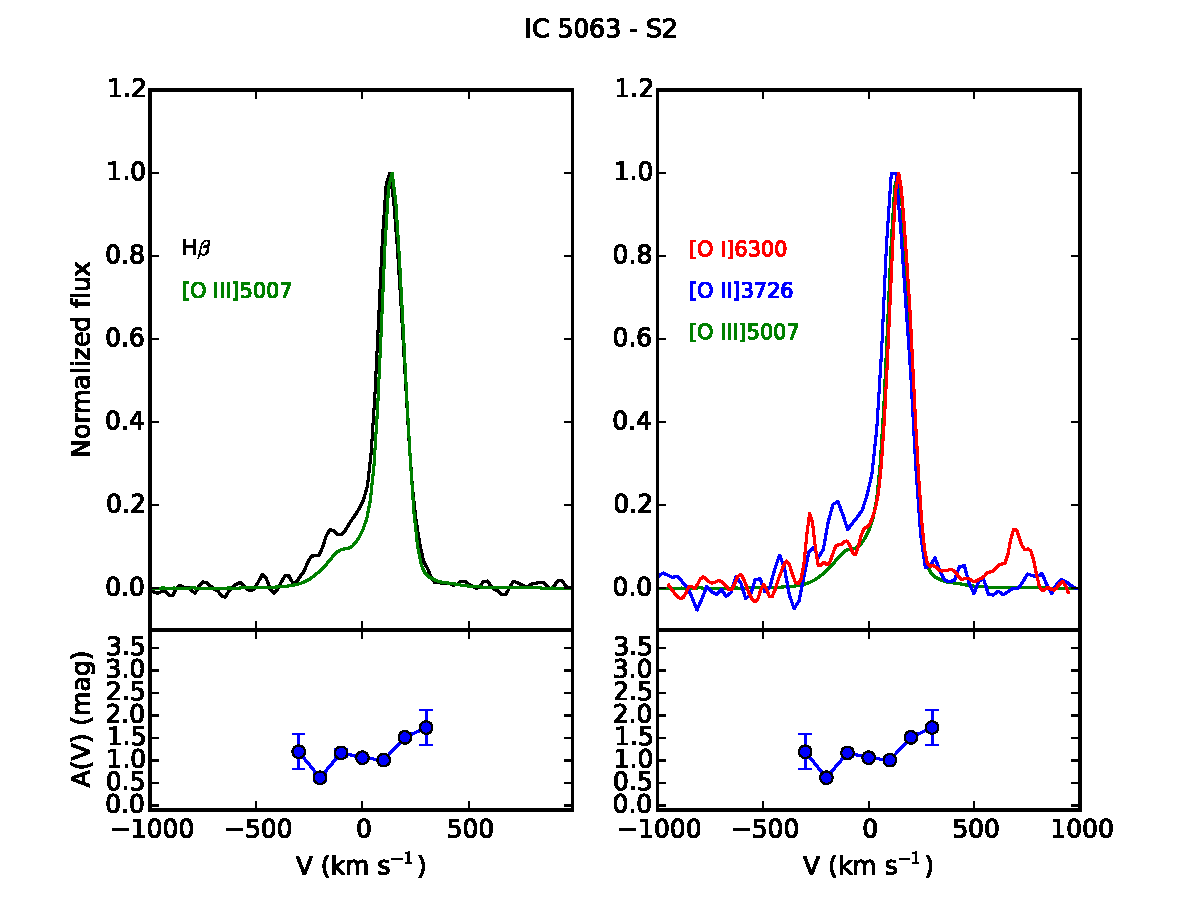
\includegraphics[width=0.45\textwidth]{images/paper1/IC5063_s2_l1.pdf} \quad
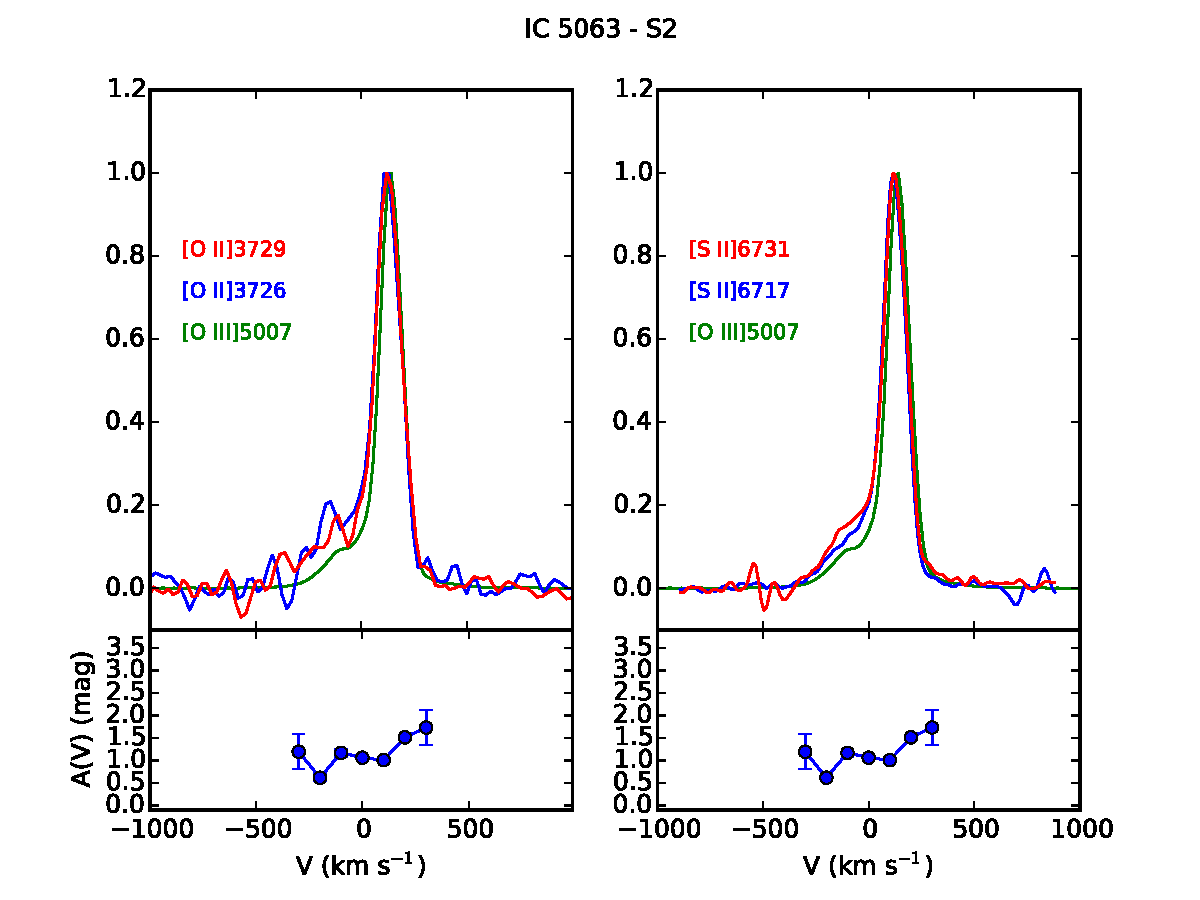
\includegraphics[width=0.45\textwidth]{images/paper1/IC5063_s2_l2.pdf}\\
\caption[]{Comparison of the emission lines of the S2 region of IC\,5063. The behaviour of the extinction coefficient as a function of velocity is shown under each plot.}
\label{fig:s2l1_I}
\end{figure*}





\newpage
\section{NGC 7212}

\begin{figure*}
\centering
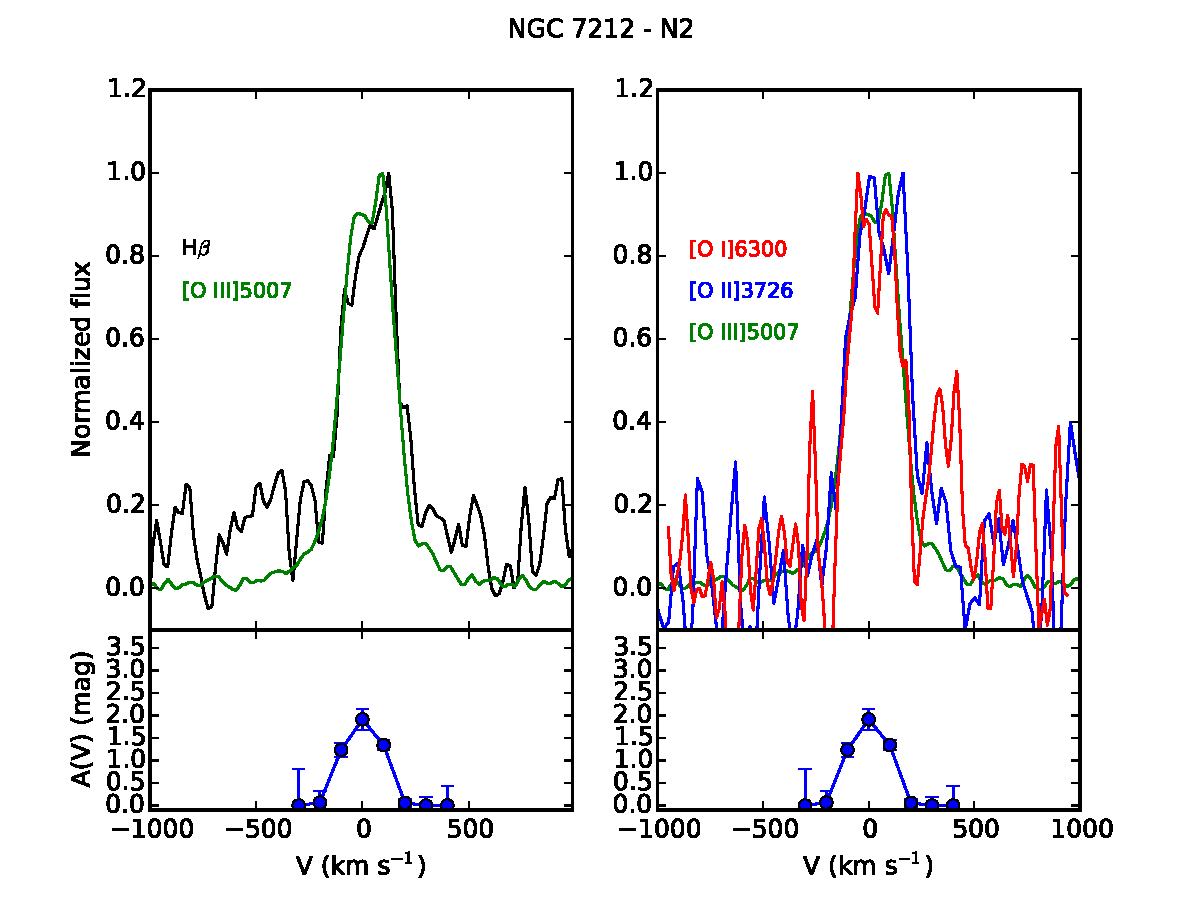
\includegraphics[width=0.45\textwidth]{images/paper1/NGC7212_n2_l1.pdf} \quad
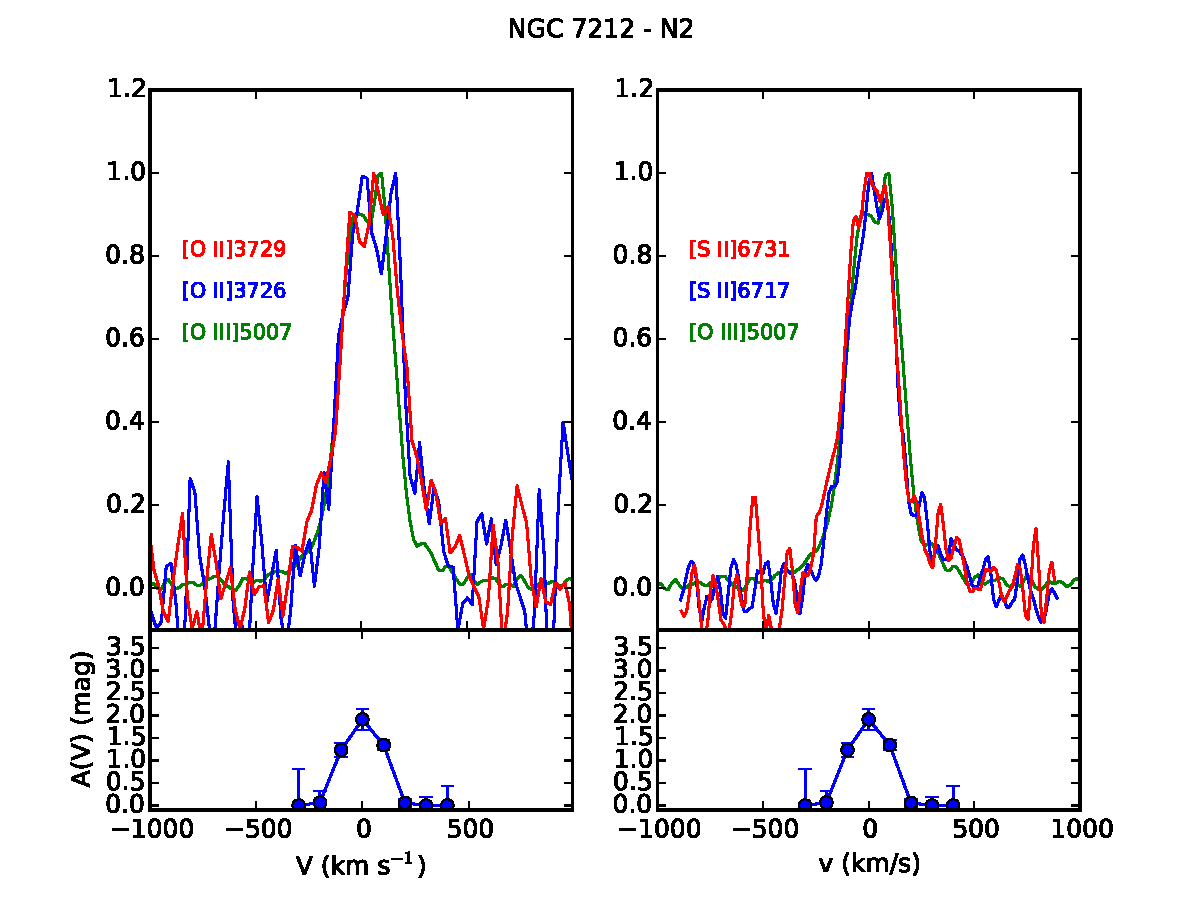
\includegraphics[width=0.45\textwidth]{images/paper1/NGC7212_n2_l2.pdf}\\
\caption[]{Comparison of the emission lines of the N2 region of NGC\,7212. The behaviour of the extinction coefficient as a function of velocity is shown under each plot.}
\label{fig:n2l1_N}
\end{figure*}



\begin{figure*}
\centering
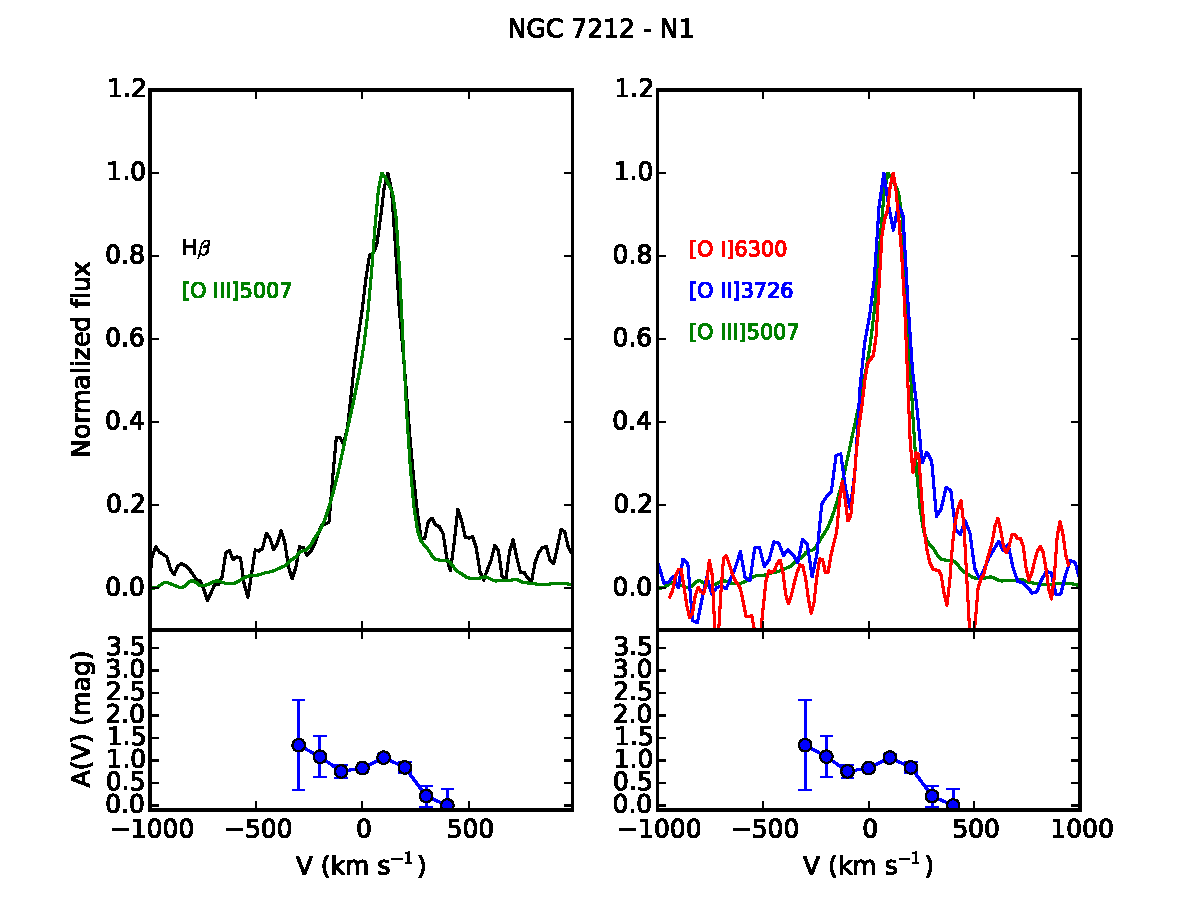
\includegraphics[width=0.45\textwidth]{images/paper1/NGC7212_n1_l1.pdf} \quad
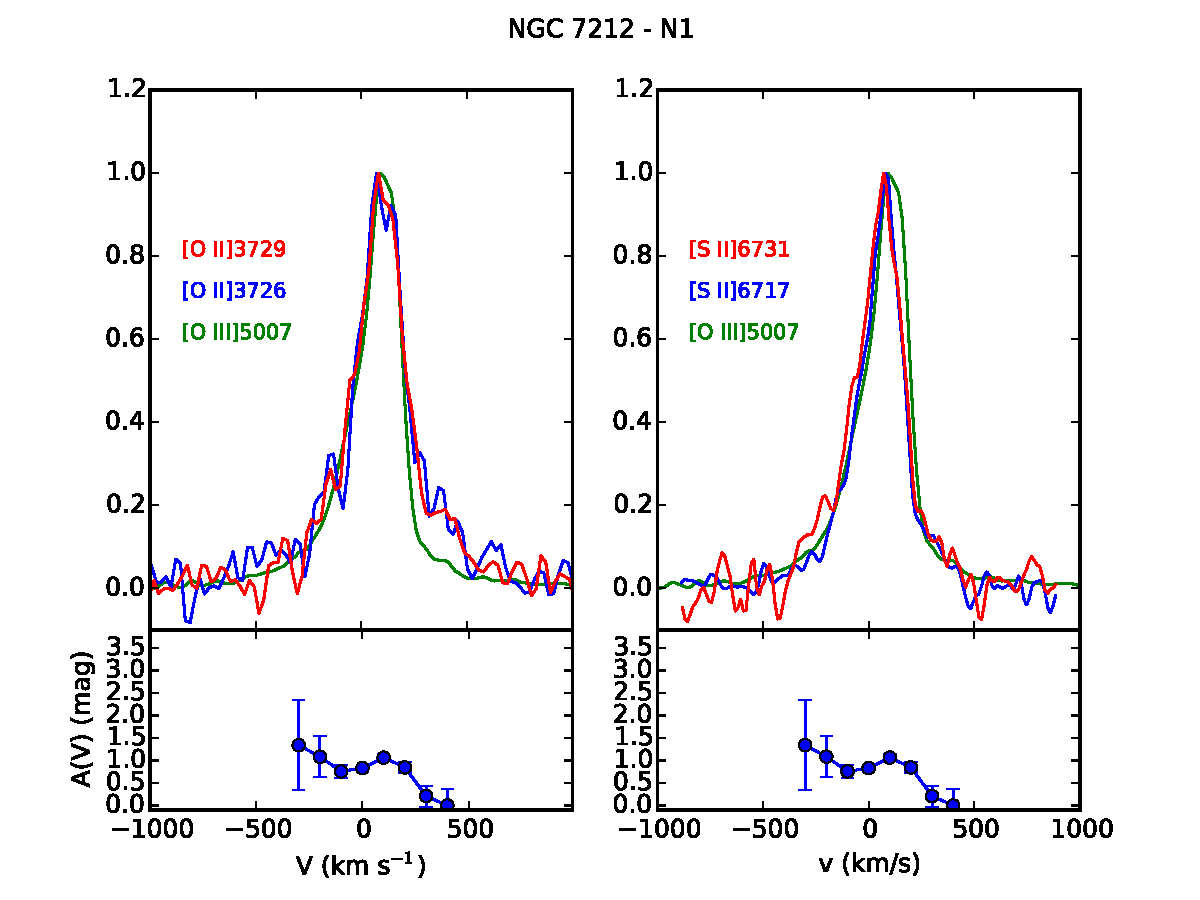
\includegraphics[width=0.45\textwidth]{images/paper1/NGC7212_n1_l2.pdf}\\
\caption[]{Comparison of the emission lines of the N1 region of NGC\,7212. The behaviour of the extinction coefficient as a function of velocity is shown under each plot.}
\label{fig:n1l1_N}
\end{figure*}

\begin{figure*}
\centering
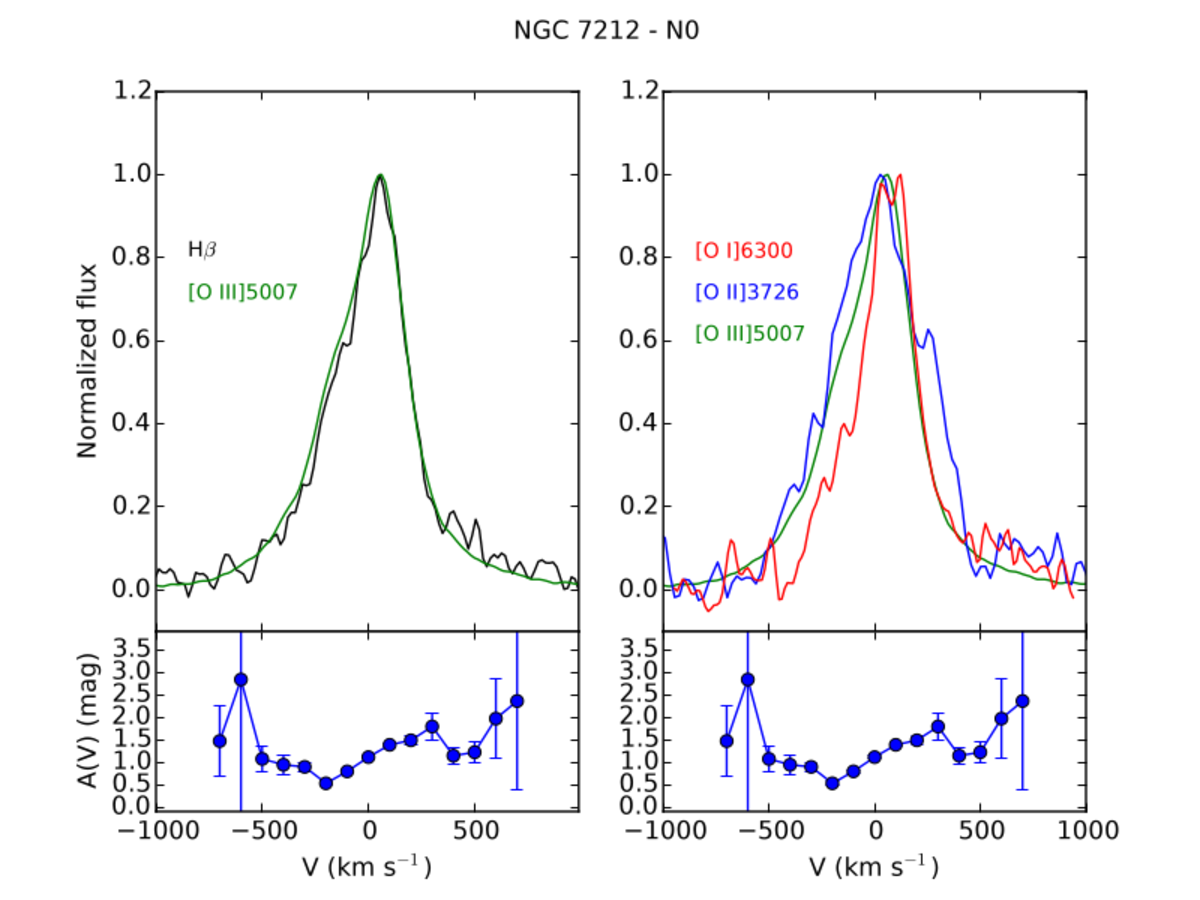
\includegraphics[width=0.45\textwidth]{images/paper1/NGC7212_n0_l1.pdf} \quad
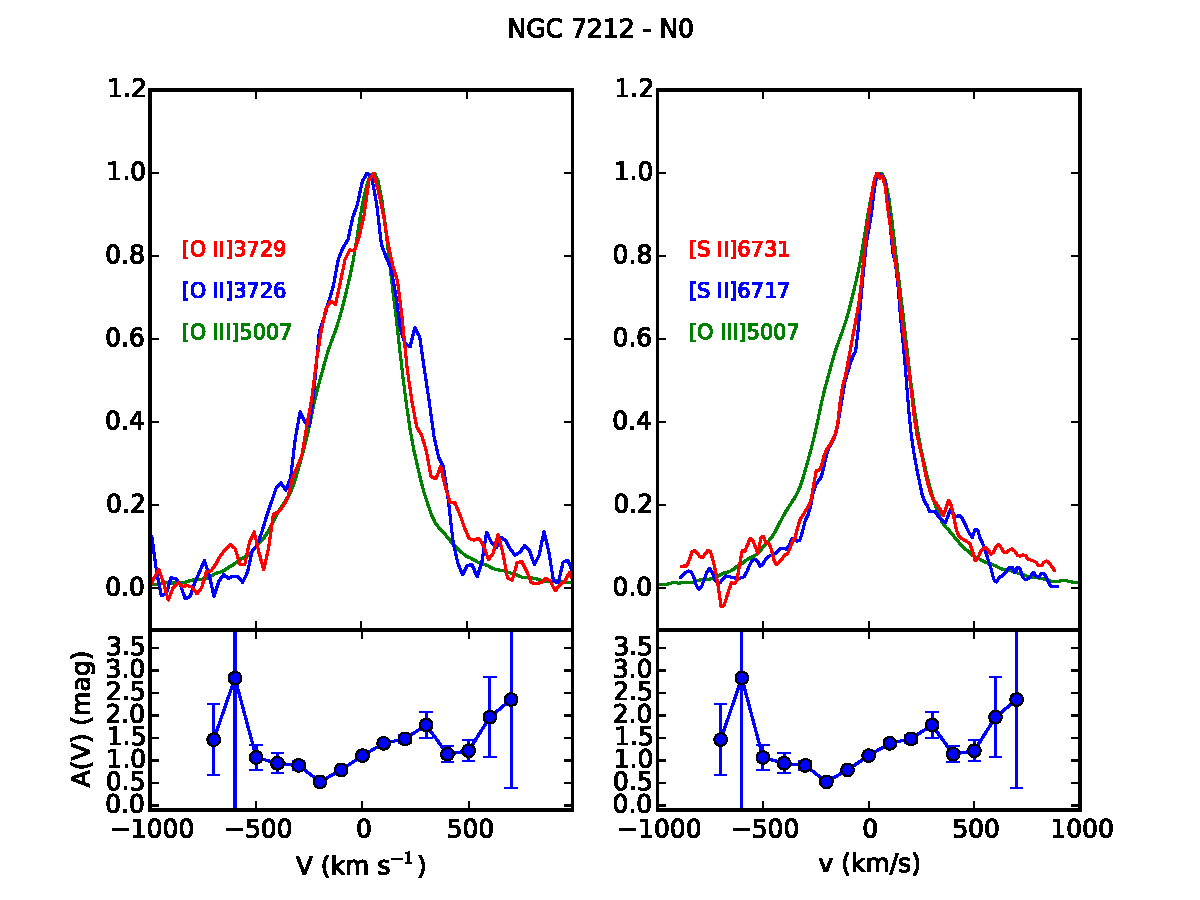
\includegraphics[width=0.45\textwidth]{images/paper1/NGC7212_n0_l2.pdf}\\
\caption[]{Comparison of the emission lines of the N0 region of NGC\,7212. The behaviour of the extinction coefficient as a function of velocity is shown under each plot.}
\label{fig:n0l1_N}
\end{figure*}


\begin{figure*}
\centering
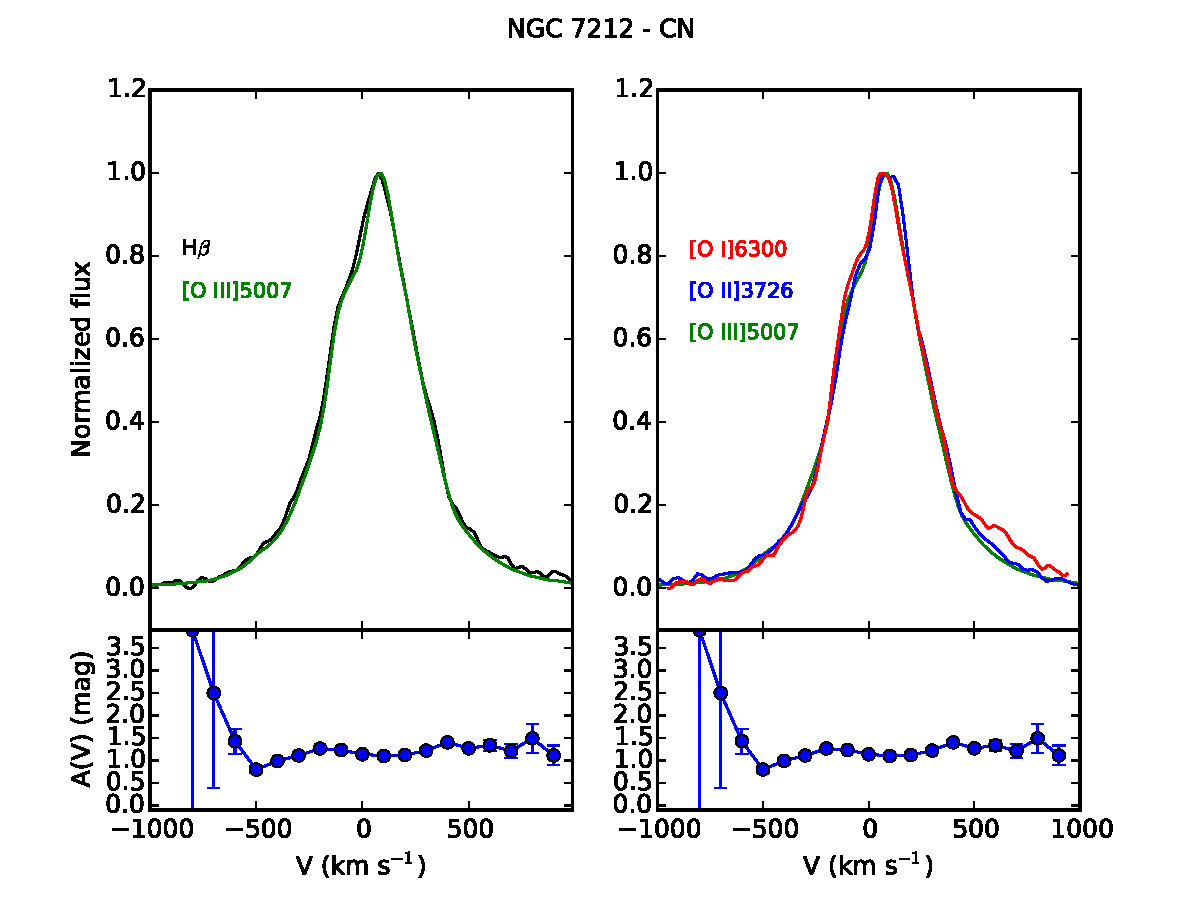
\includegraphics[width=0.45\textwidth]{images/paper1/NGC7212_cn_l1.pdf} \quad
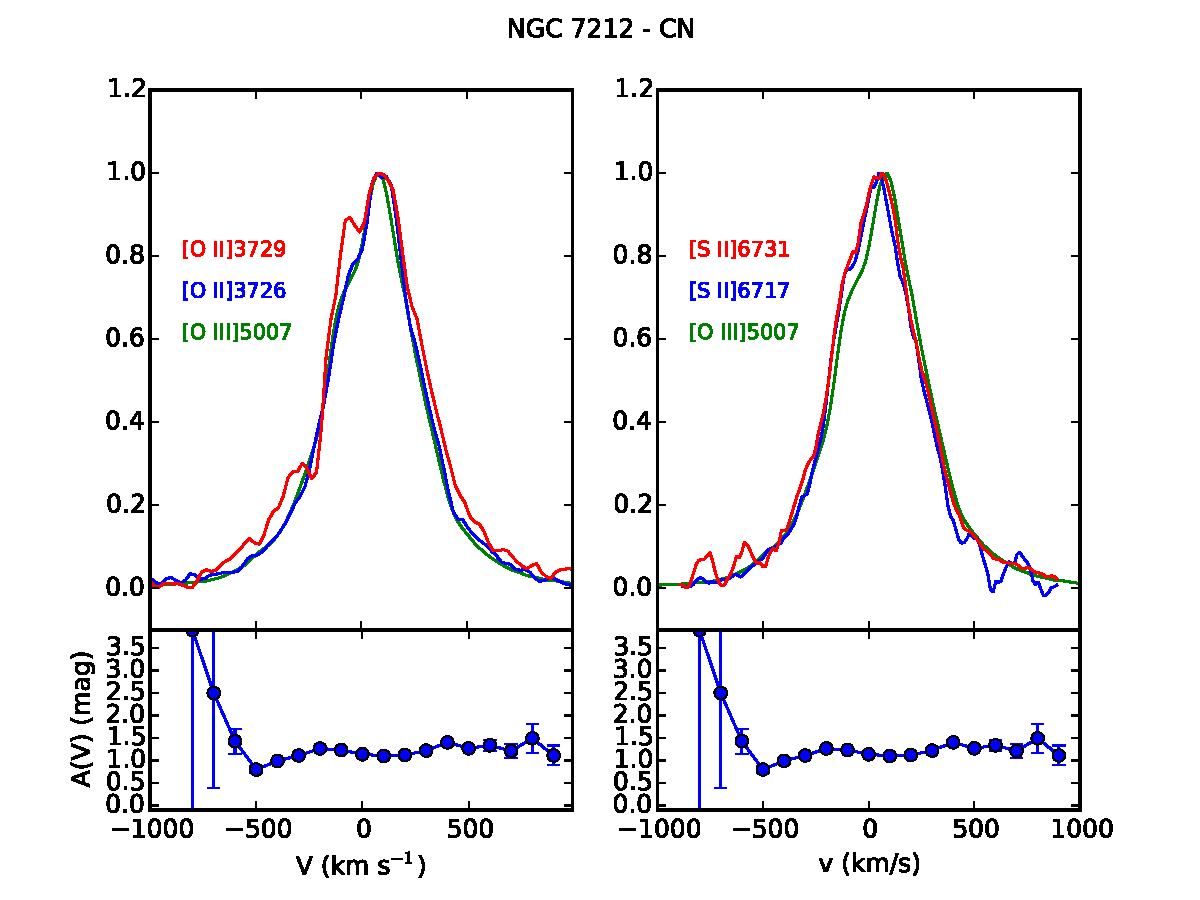
\includegraphics[width=0.45\textwidth]{images/paper1/NGC7212_cn_l2.pdf}\\
\caption[]{Comparison of the emission lines of the CN region of NGC\,7212. The behaviour of the extinction coefficient as a function of velocity is shown under each plot.}
\label{fig:cnl1_N}
\end{figure*}

\begin{figure*}
\centering
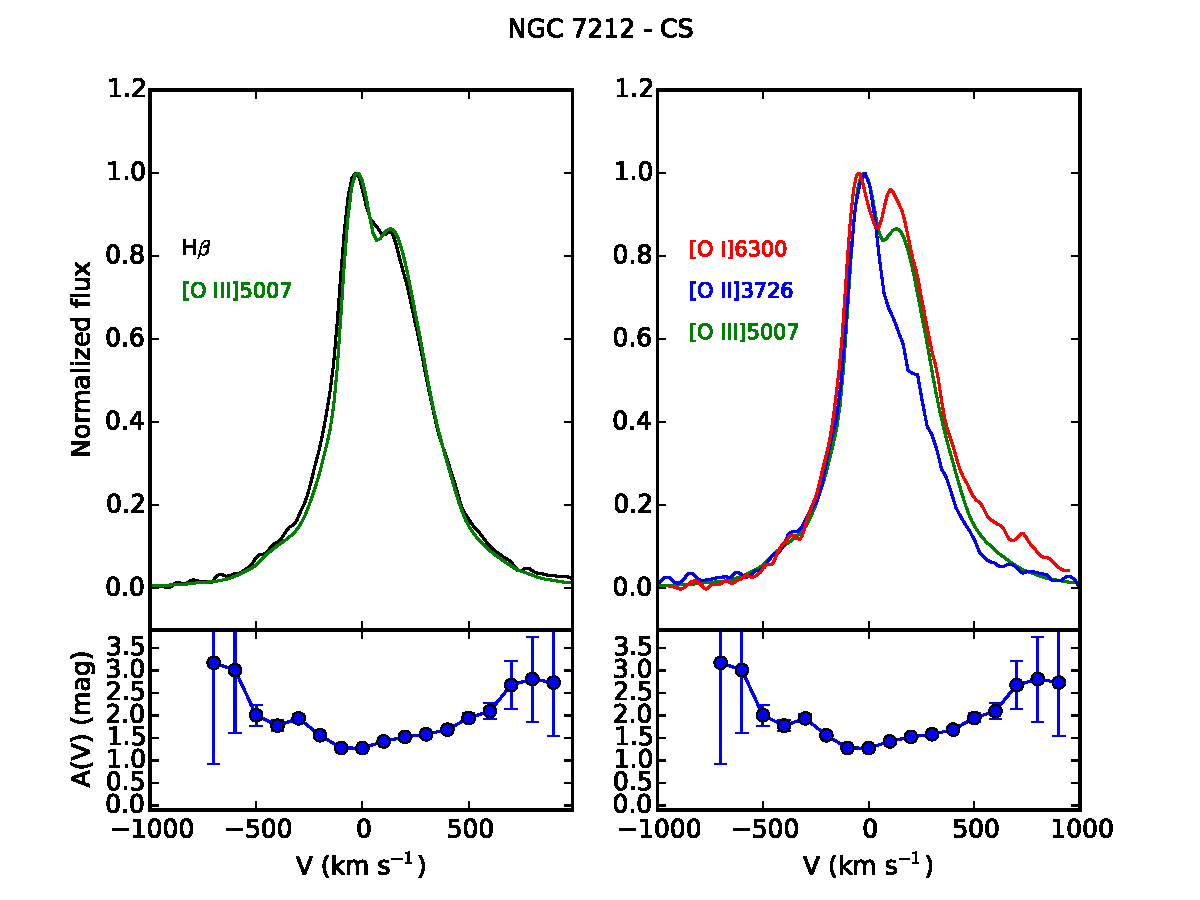
\includegraphics[width=0.45\textwidth]{images/paper1/NGC7212_cs_l1.pdf} \quad
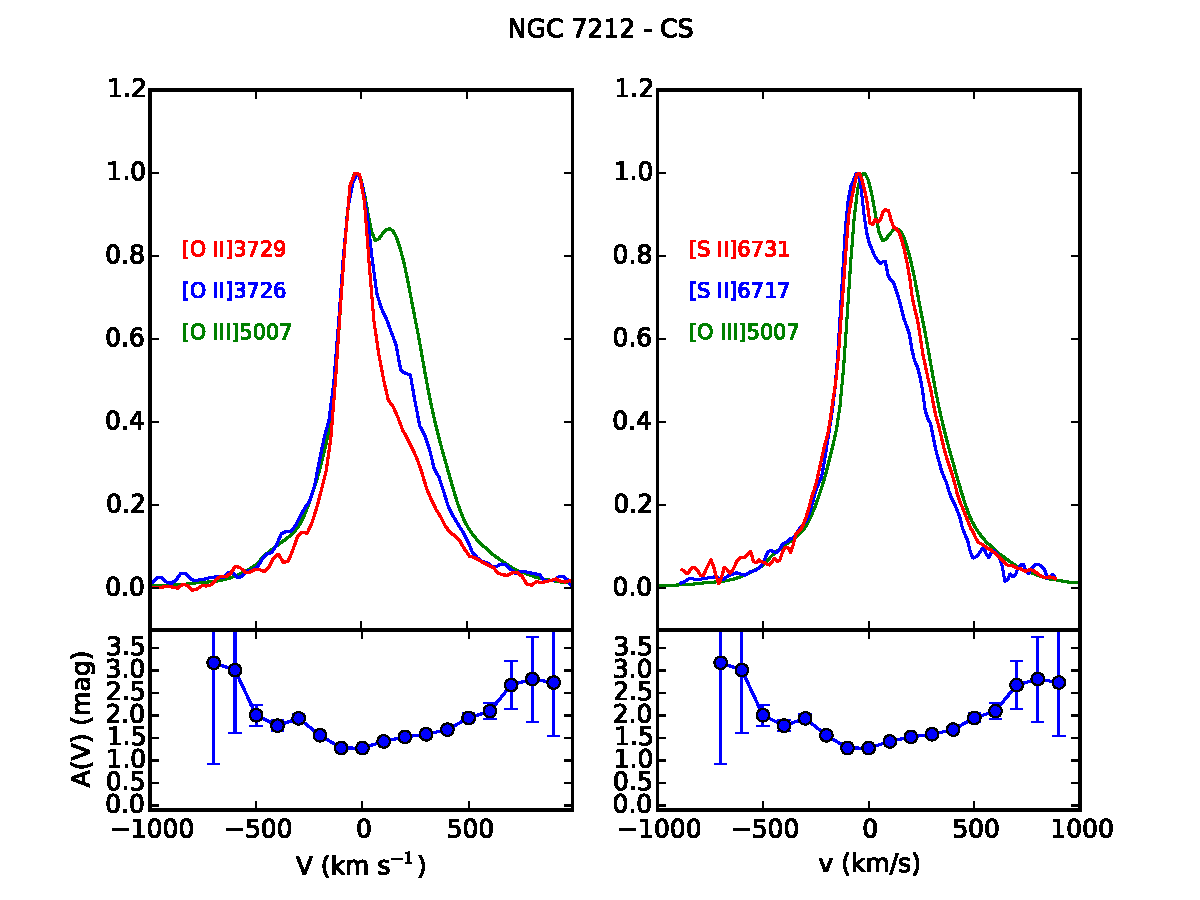
\includegraphics[width=0.45\textwidth]{images/paper1/NGC7212_cs_l2.pdf}\\
\caption[]{Comparison of the emission lines of the CS region of NGC\,7212. The behaviour of the extinction coefficient as a function of velocity is shown under each plot.}
\label{fig:csl1_N}
\end{figure*}

\begin{figure*}
\centering
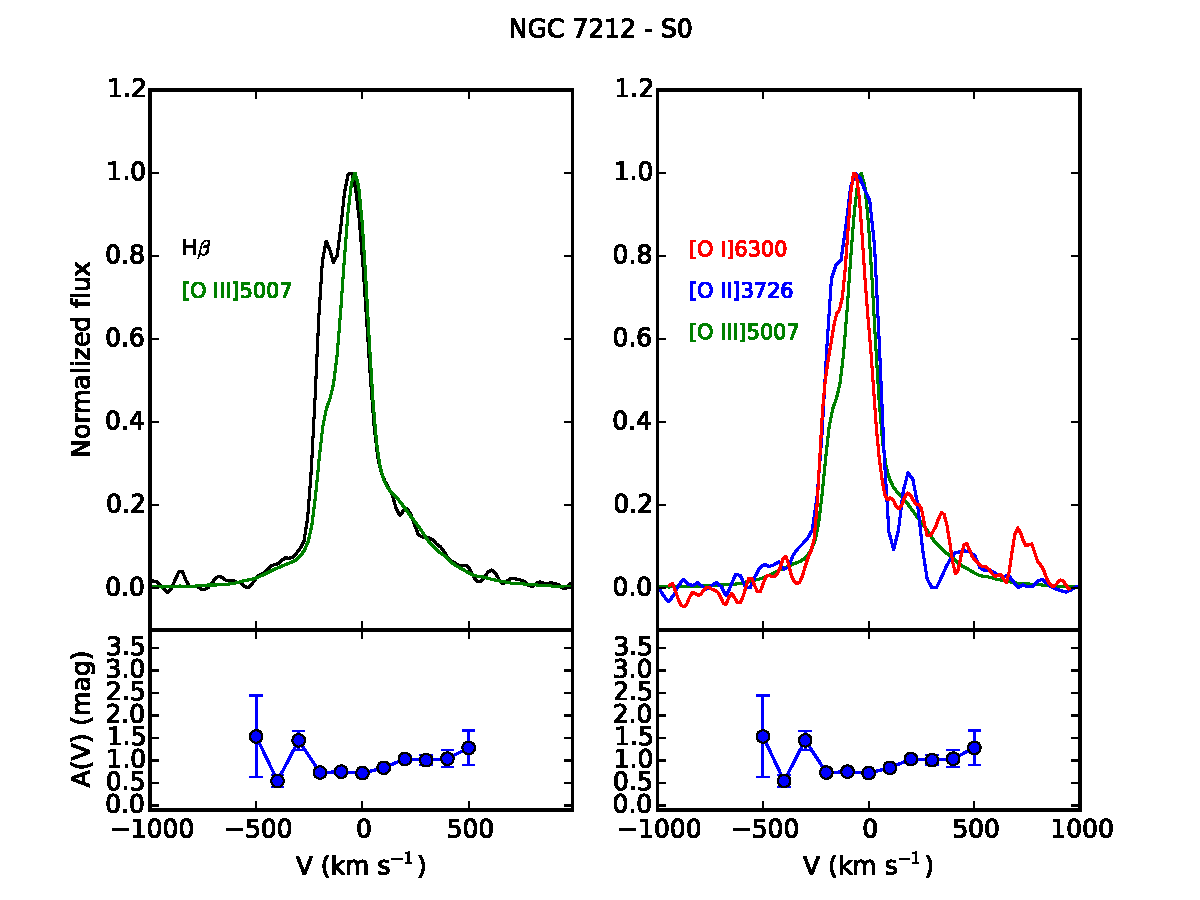
\includegraphics[width=0.45\textwidth]{images/paper1/NGC7212_s0_l1.pdf} \quad
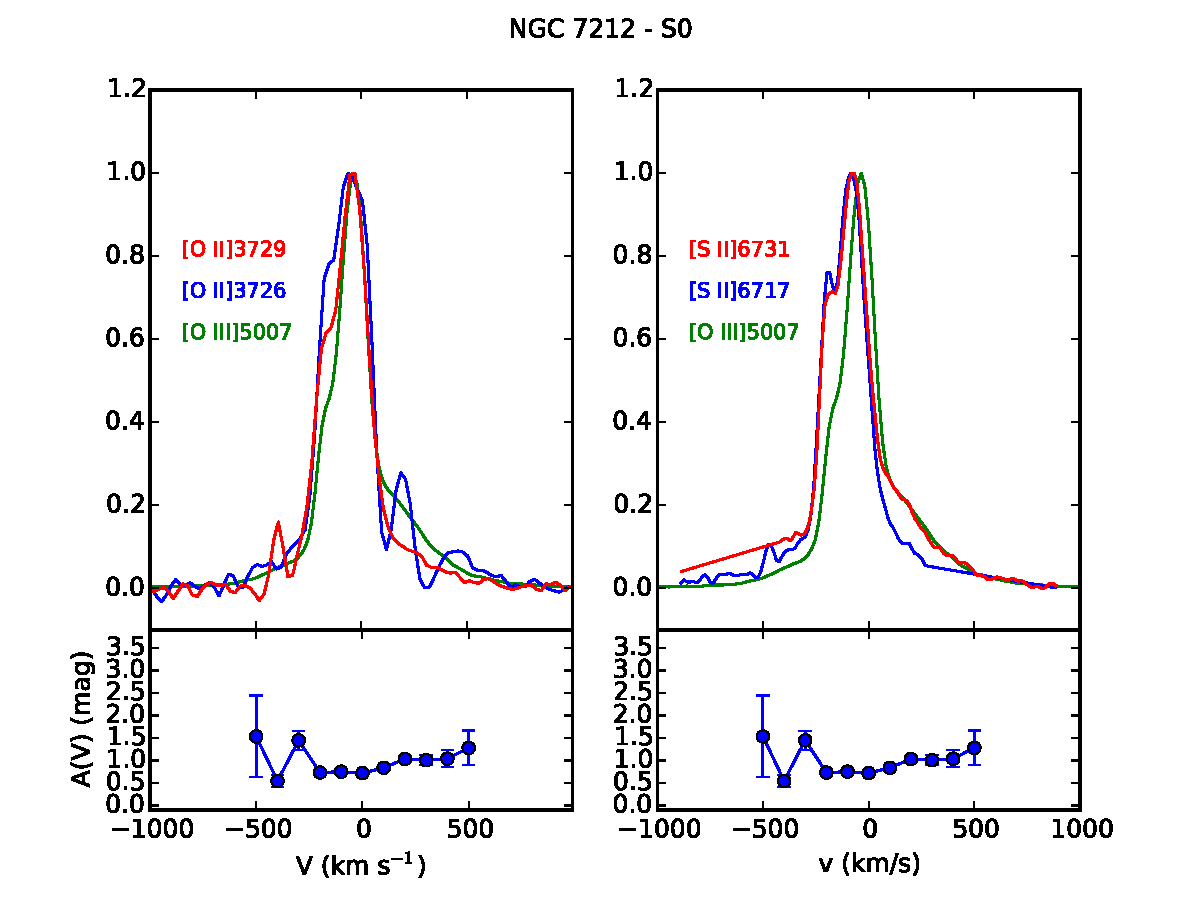
\includegraphics[width=0.45\textwidth]{images/paper1/NGC7212_s0_l2.pdf}\\
\caption[]{Comparison of the emission lines of the S0 region of NGC\,7212. The behaviour of the extinction coefficient as a function of velocity is shown under each plot.}
\label{fig:s0l1_N}
\end{figure*}

\begin{figure*}
\centering
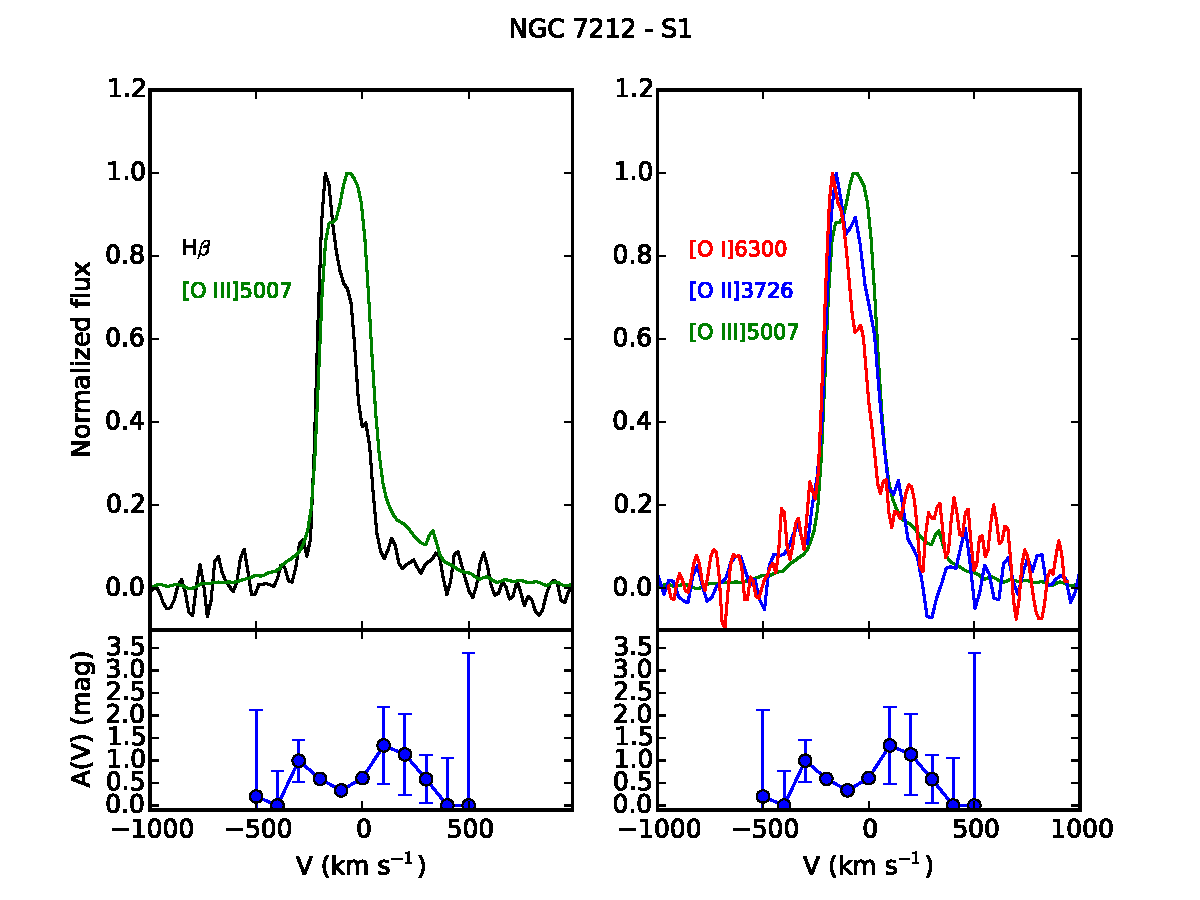
\includegraphics[width=0.45\textwidth]{images/paper1/NGC7212_s1_l1.pdf} \quad
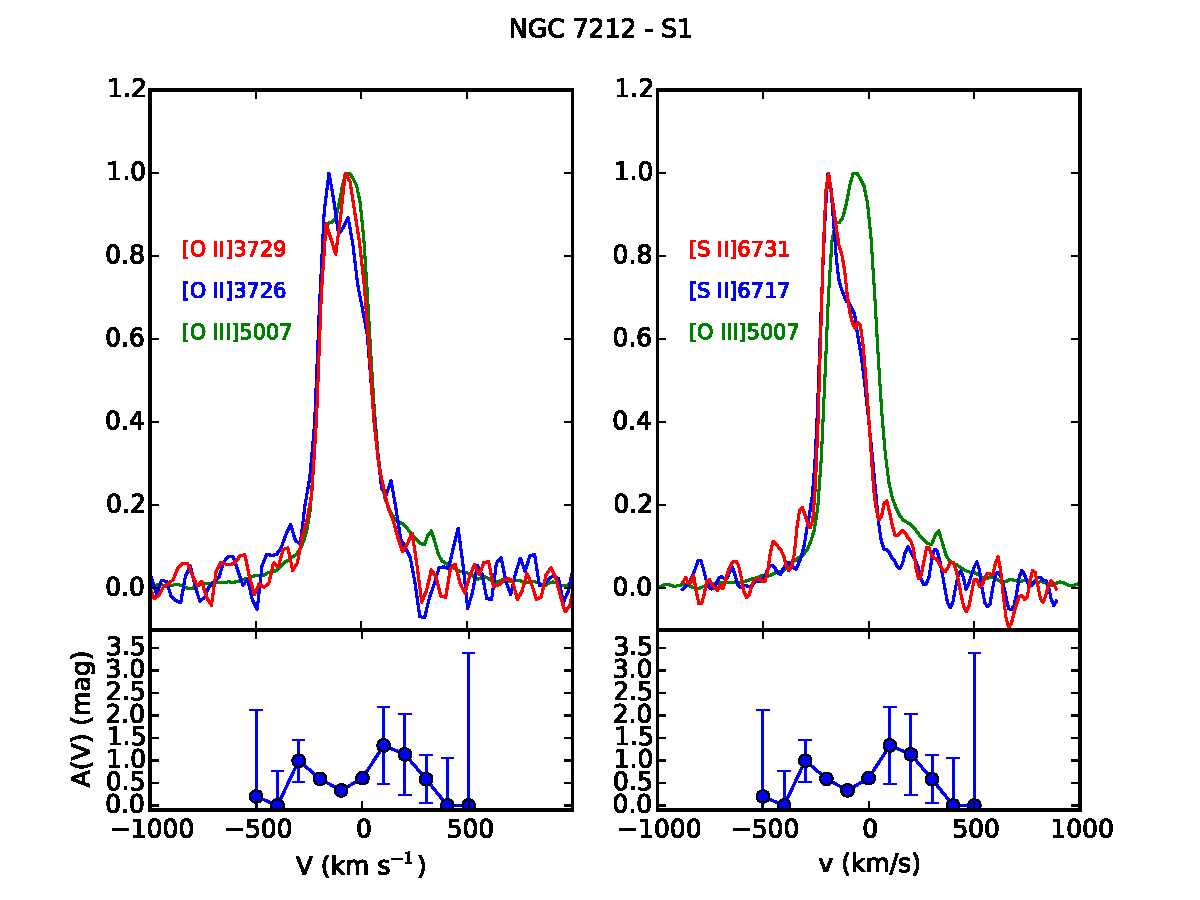
\includegraphics[width=0.45\textwidth]{images/paper1/NGC7212_s1_l2.pdf}\\
\caption[]{Comparison of the emission lines of the S1 region of NGC\,7212. The behaviour of the extinction coefficient as a function of velocity is shown under each plot.}
\label{fig:s1l1_N}
\end{figure*}

\section{Diagnostic Diagrams}
\label{sec:Adiag}

\begin{figure*} 
\centering
\subfloat[][]{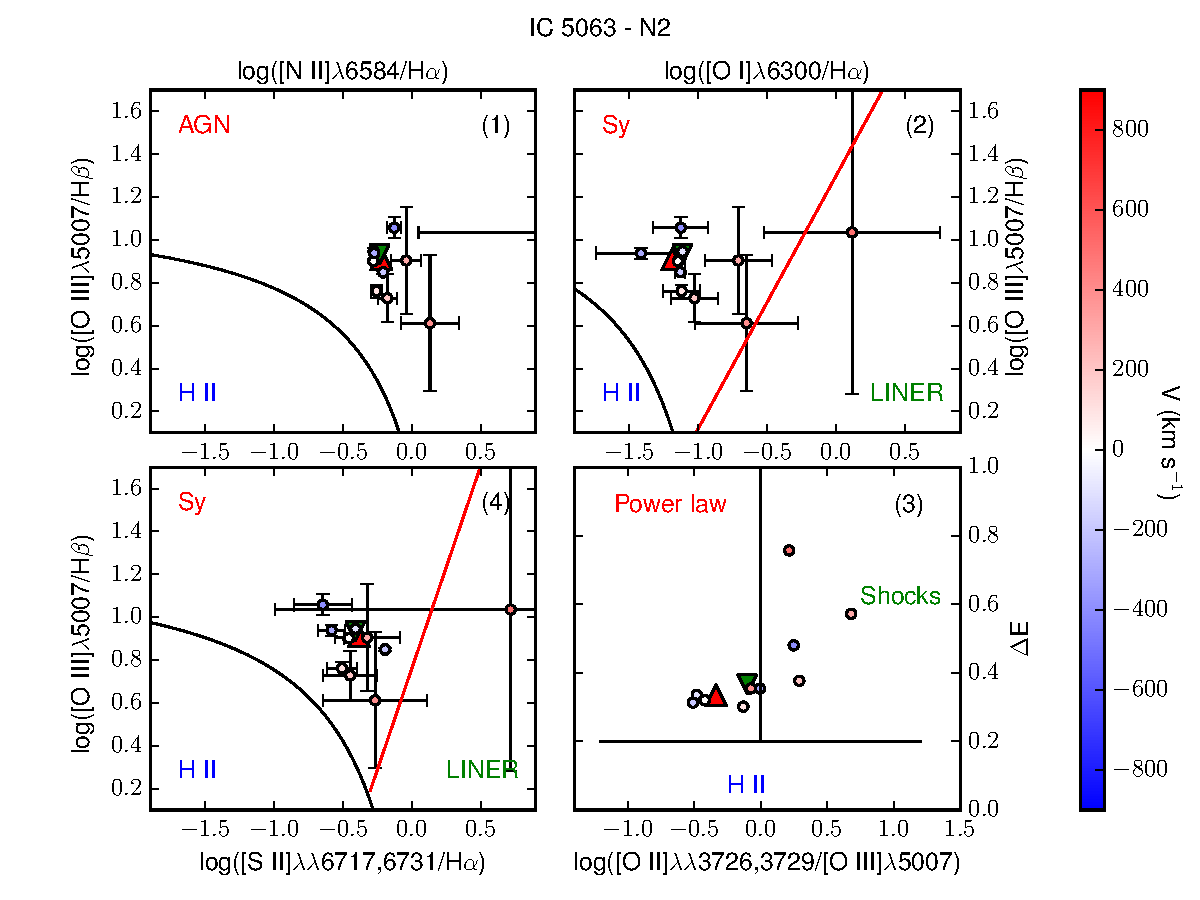
\includegraphics[width=0.43\textwidth]{images/paper1/IC5063_n2_diag.pdf}} \quad
\subfloat[][]{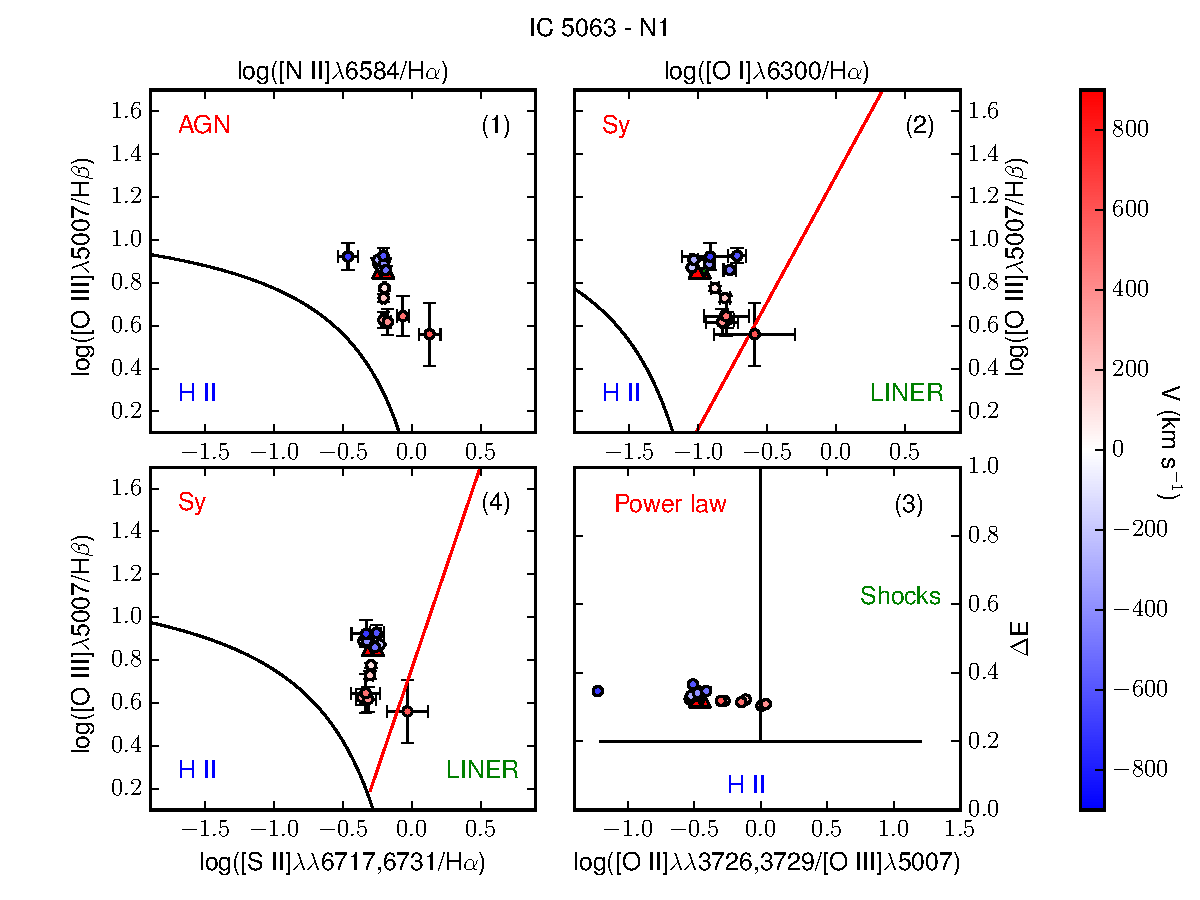
\includegraphics[width=0.43\textwidth]{images/paper1/IC5063_n1_diag.pdf}}\\
\subfloat[][]{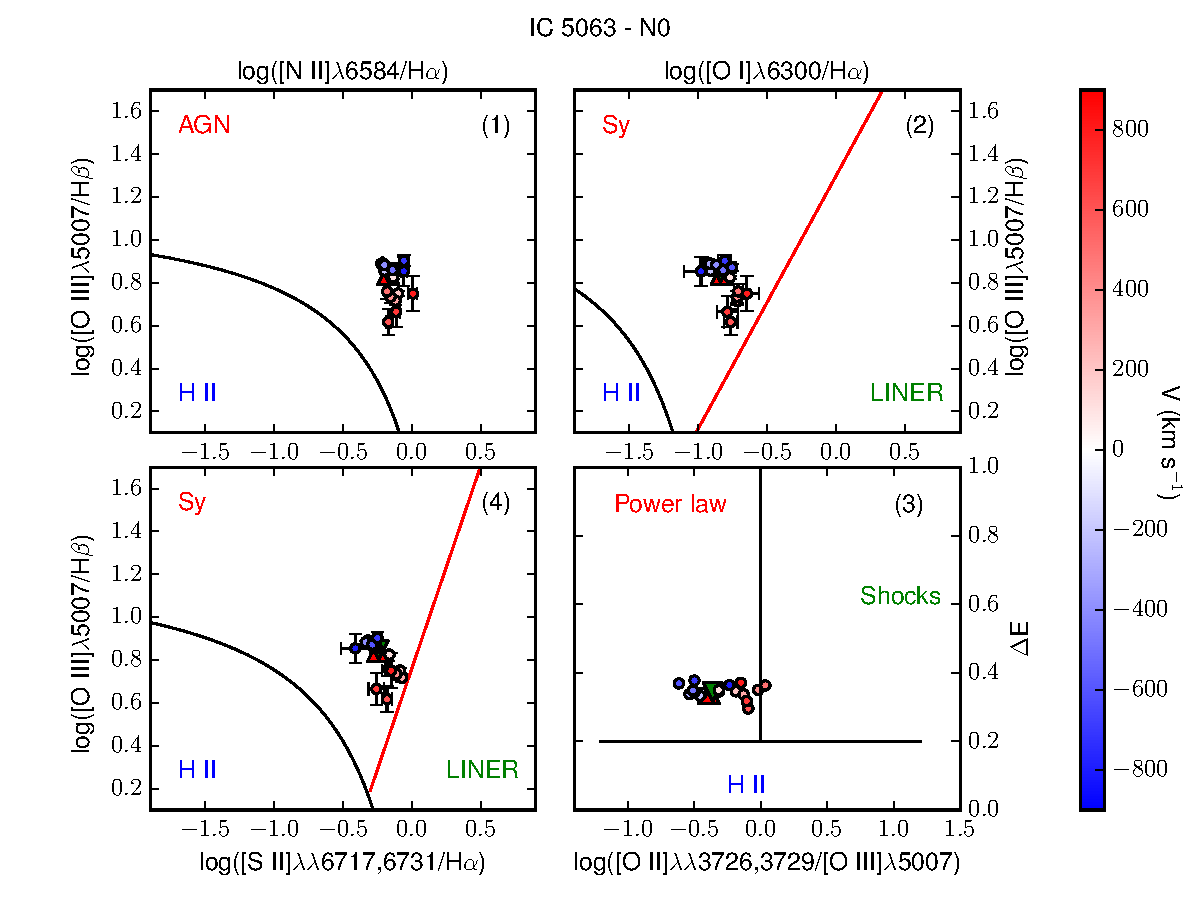
\includegraphics[width=0.43\textwidth]{images/paper1/IC5063_n0_diag.pdf}} \quad
\subfloat[][]{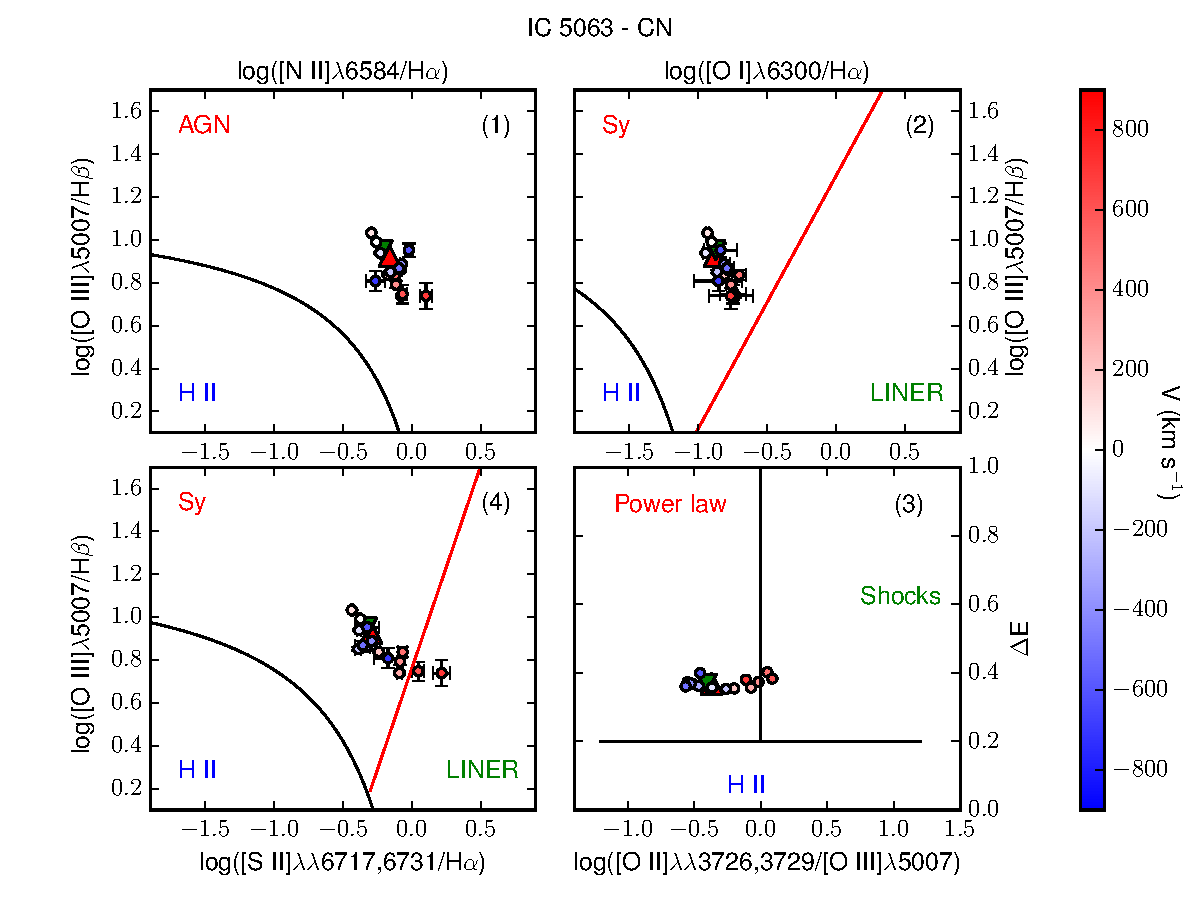
\includegraphics[width=0.43\textwidth]{images/paper1/IC5063_cn_diag.pdf}}\\
\subfloat[][]{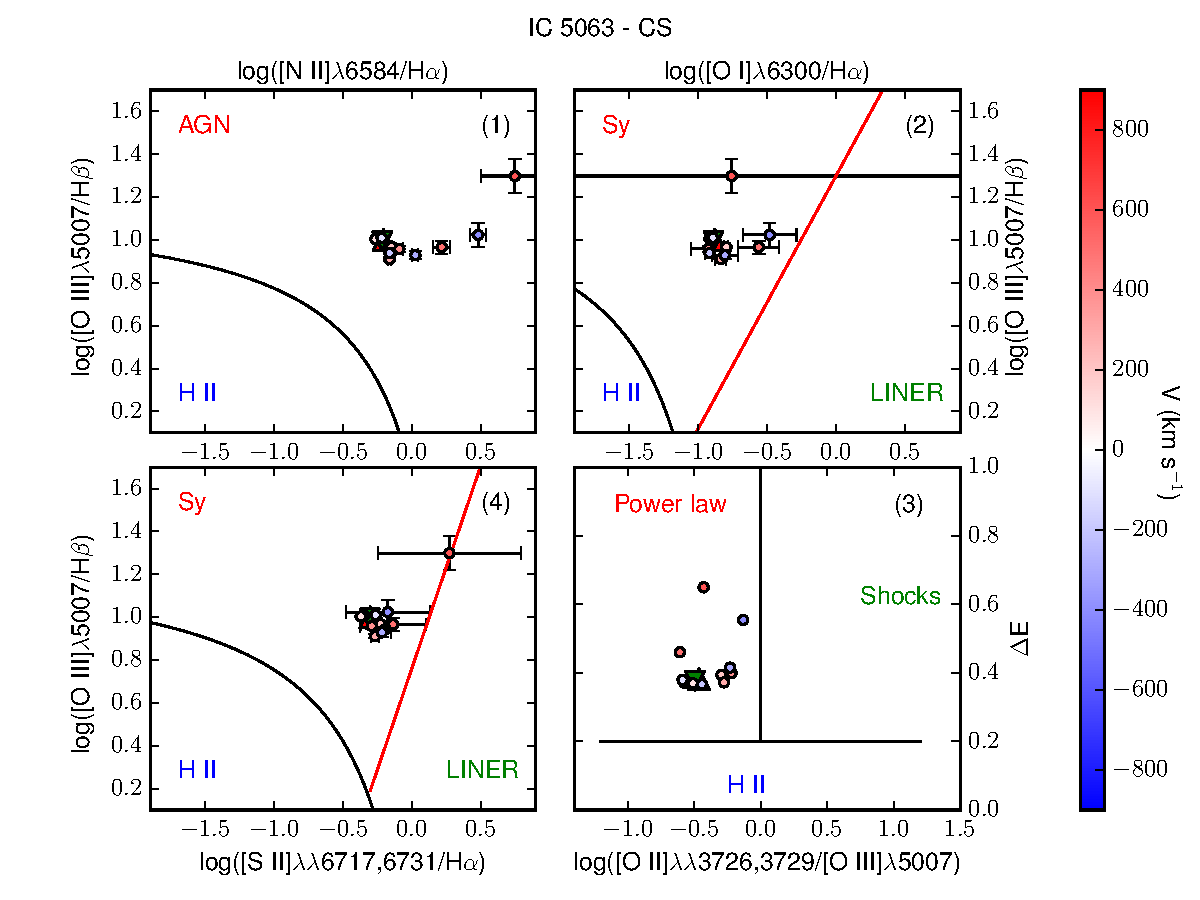
\includegraphics[width=0.43\textwidth]{images/paper1/IC5063_cs_diag.pdf}} \quad
\subfloat[][]{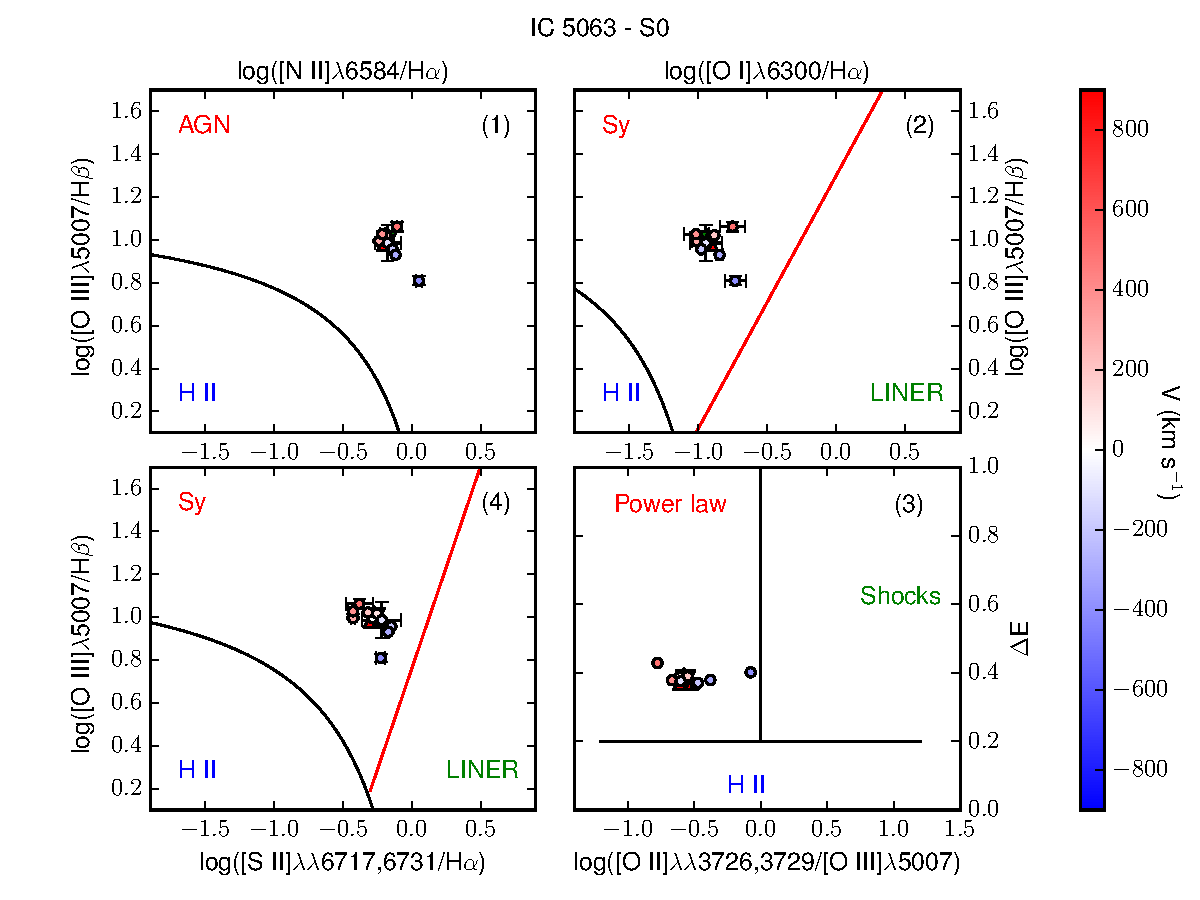
\includegraphics[width=0.43\textwidth]{images/paper1/IC5063_s0_diag.pdf}}\\
\caption[]{Diagnostic diagrams of the (a) N2, (b) N1, (c) N0, (d) CN, (e) CS and (f) S0 regions of IC\,5063.  In each plot we show, from the top left panel clockwise: (1) $\log([\ion{O}{III}] \Hb)$ vs $\log([\ion{N}{II}]/ \Ha)$, (2) $\log([\ion{O}{III}]/ \Hb)$ vs $\log([\ion{O}{I}]/ \Ha)$, (3) $\Delta E$ vs $\log([\ion{O}{II}]/[\ion{O}{III}])$, (4) $\log([\ion{O}{III}]/ \Hb)$ vs $\log([\ion{S}{II}]/ \Ha)$ \citep{Baldwin81, Veilleux87}. The colorbar shows the velocity of each bin. The black curves in (1), (2), (4) divide power-law ionized regions (top) and HII regions (bottom). The red lines divide Seyfert-like regions (left) and LINER-like regions (right) \citep{Kewley06}. The black lines in (3) divide HII regions (bottom), power-law ionized region (left) and shock ionized regions (right) \citep{Baldwin81}.  }
\label{fig:diag_css0}
\end{figure*}

\begin{figure*} 
\centering
\subfloat[][]{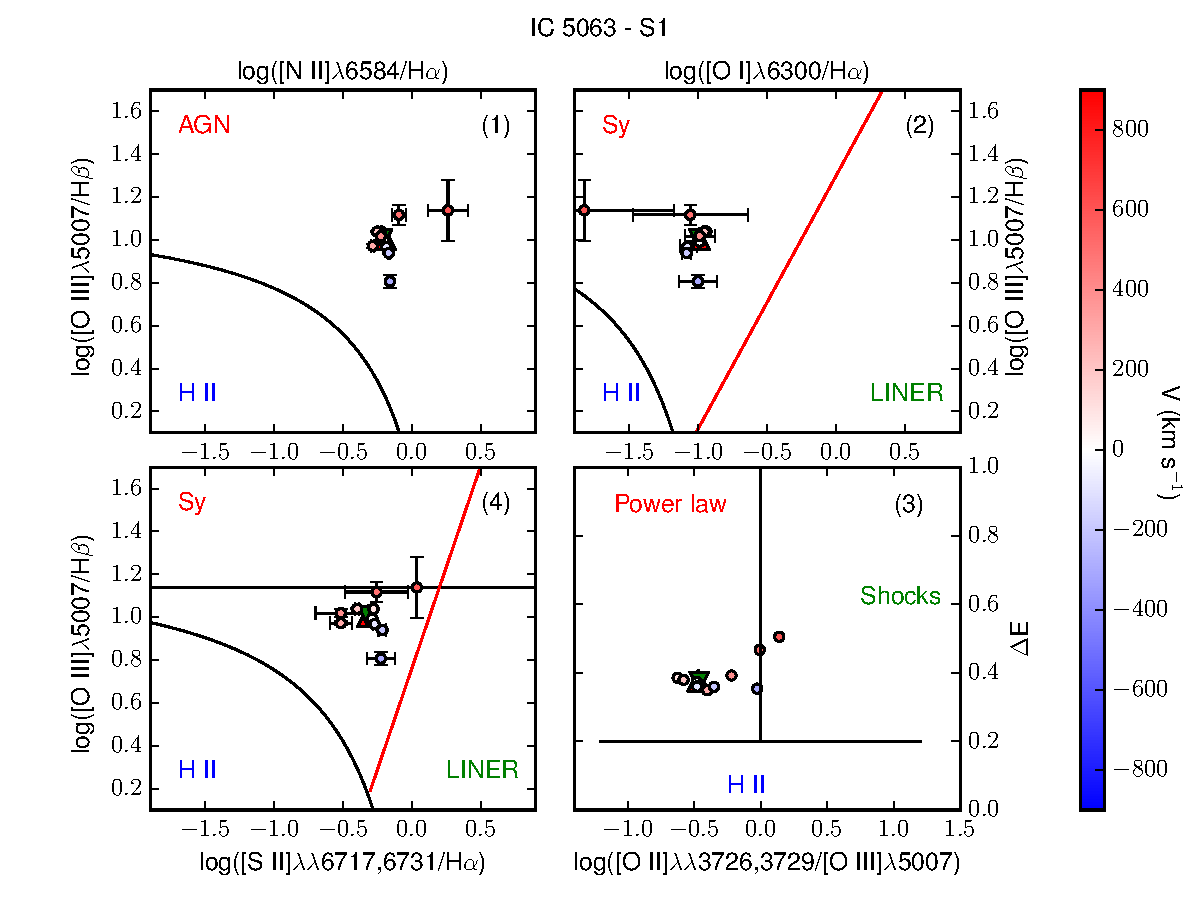
\includegraphics[width=0.43\textwidth]{images/paper1/IC5063_s1_diag.pdf}} \quad
\subfloat[][]{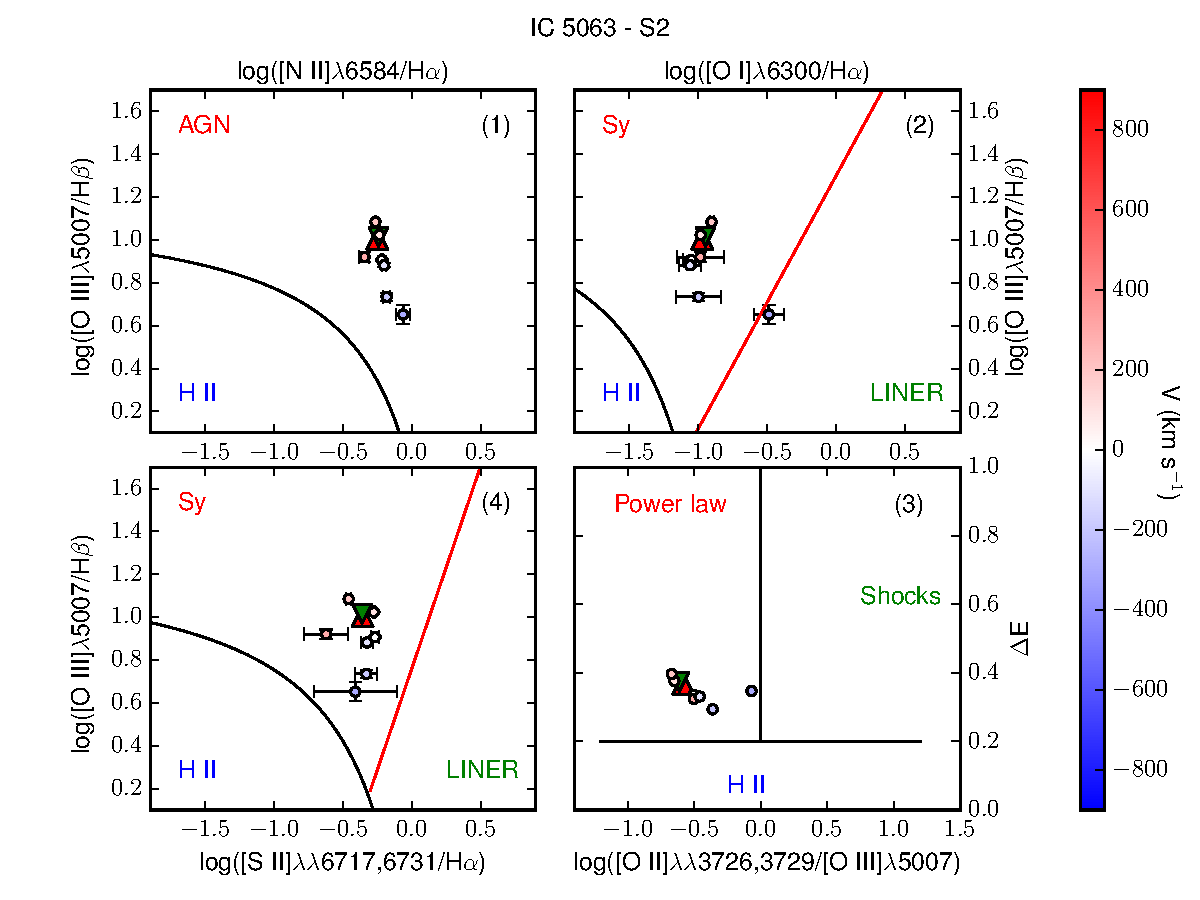
\includegraphics[width=0.43\textwidth]{images/paper1/IC5063_s2_diag.pdf}}\\
\subfloat[][]{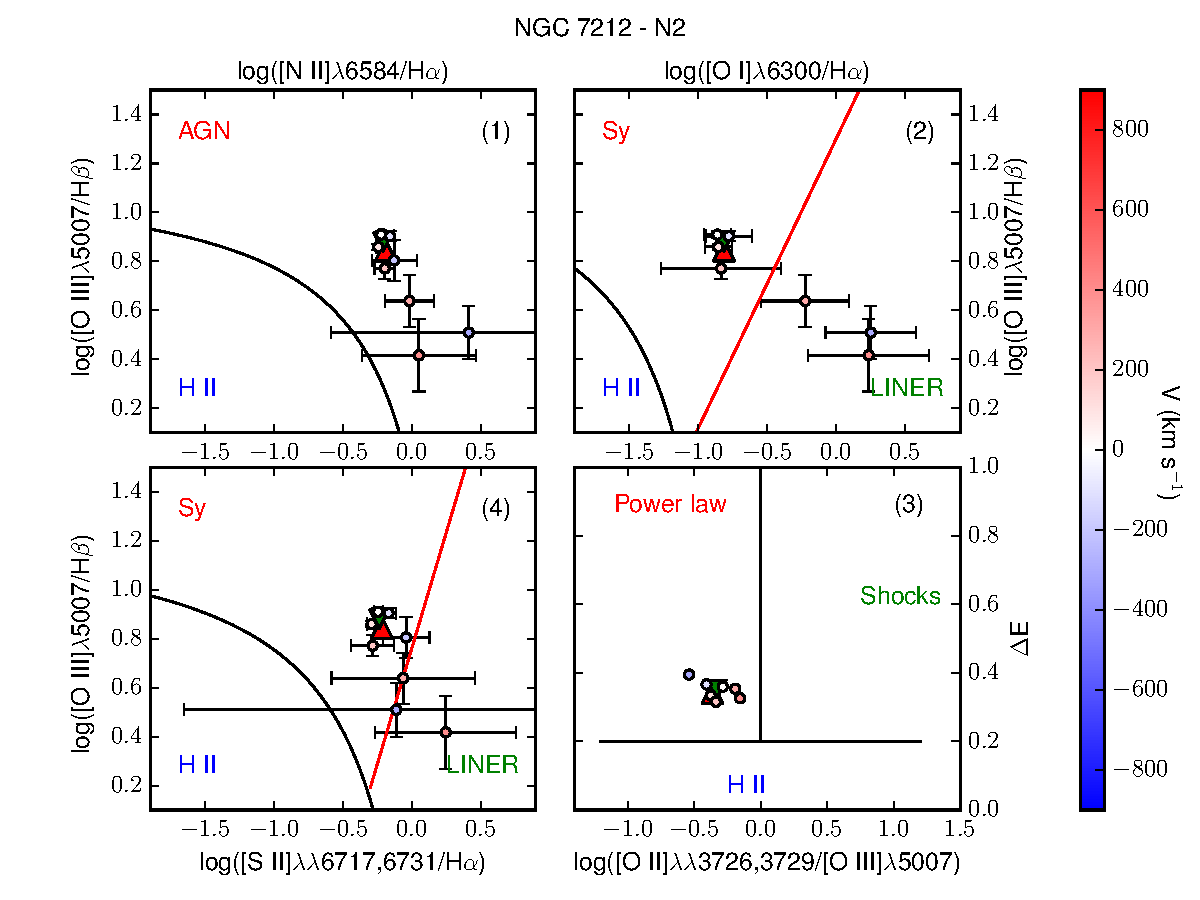
\includegraphics[width=0.43\textwidth]{images/paper1/NGC7212_n2_diag.pdf}} \quad
\subfloat[][]{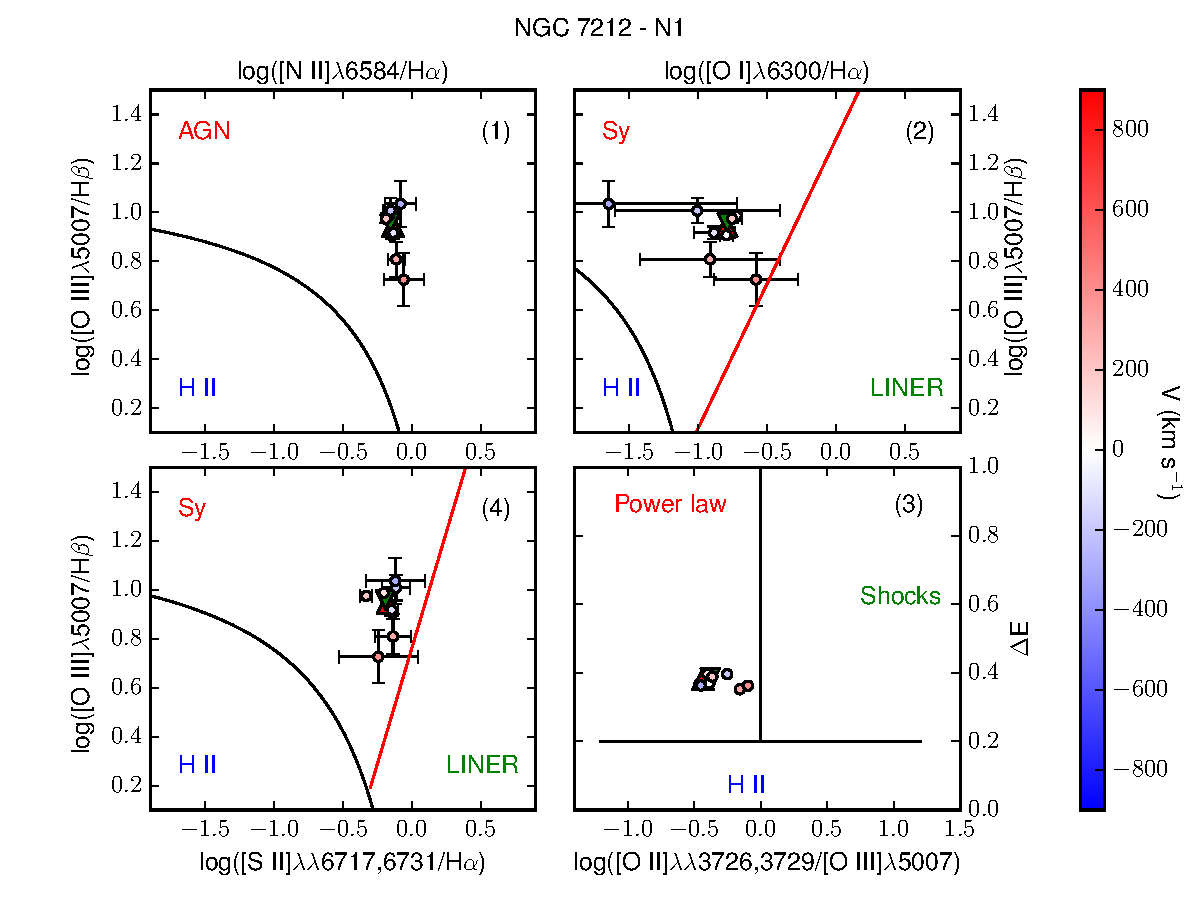
\includegraphics[width=0.43\textwidth]{images/paper1/NGC7212_n1_diag.pdf}}\\
\subfloat[][]{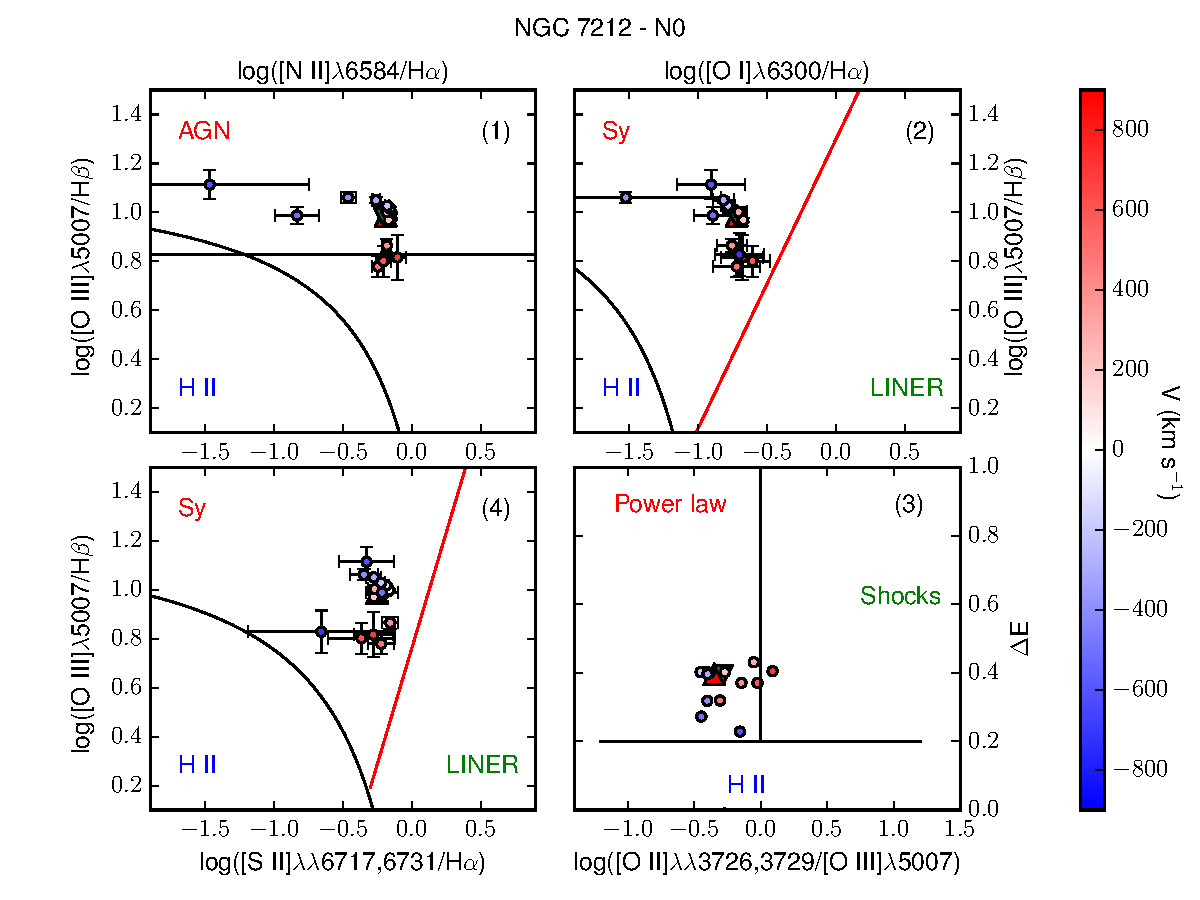
\includegraphics[width=0.43\textwidth]{images/paper1/NGC7212_n0_diag.pdf}} \quad
\subfloat[][]{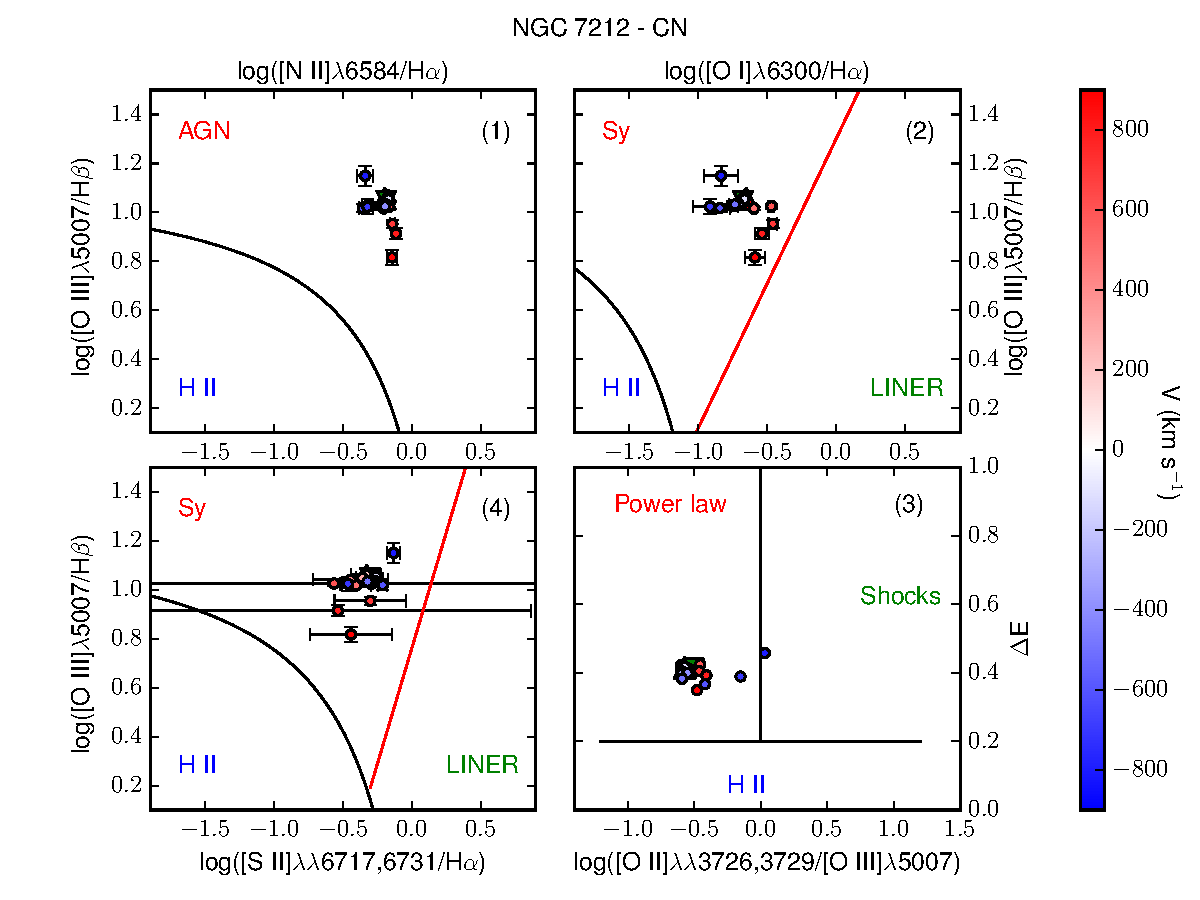
\includegraphics[width=0.43\textwidth]{images/paper1/NGC7212_cn_diag.pdf}}\\
\caption[]{Diagnostic diagrams of the (a) S1 and (b) S2 regions of IC\,5063 and (c) N2, (d) N1, (e) N0 and (f) CN  regions of NGC\,7212.  In each plot we show, from the top left panel clockwise: (1) $\log([\ion{O}{III}] \Hb)$ vs $\log([\ion{N}{II}]/ \Ha)$, (2) $\log([\ion{O}{III}]/ \Hb)$ vs $\log([\ion{O}{I}]/ \Ha)$, (3) $\Delta E$ vs $\log([\ion{O}{II}]/[\ion{O}{III}])$, (4) $\log([\ion{O}{III}]/ \Hb)$ vs $\log([\ion{S}{II}]/ \Ha)$ \citep{Baldwin81, Veilleux87}. The colorbar shows the velocity of each bin. The black curves in (1), (2), (4) divide power-law ionized regions (top) and HII regions (bottom). The red lines divide Seyfert-like regions (left) and LINER-like regions (right) \citep{Kewley06}. The black lines in (3) divide HII regions (bottom), power-law ionized region (left) and shock ionized regions (right) \citep{Baldwin81}.   }
\label{fig:diag_n0cnN}
\end{figure*}


\begin{figure*}
\centering
\subfloat[][]{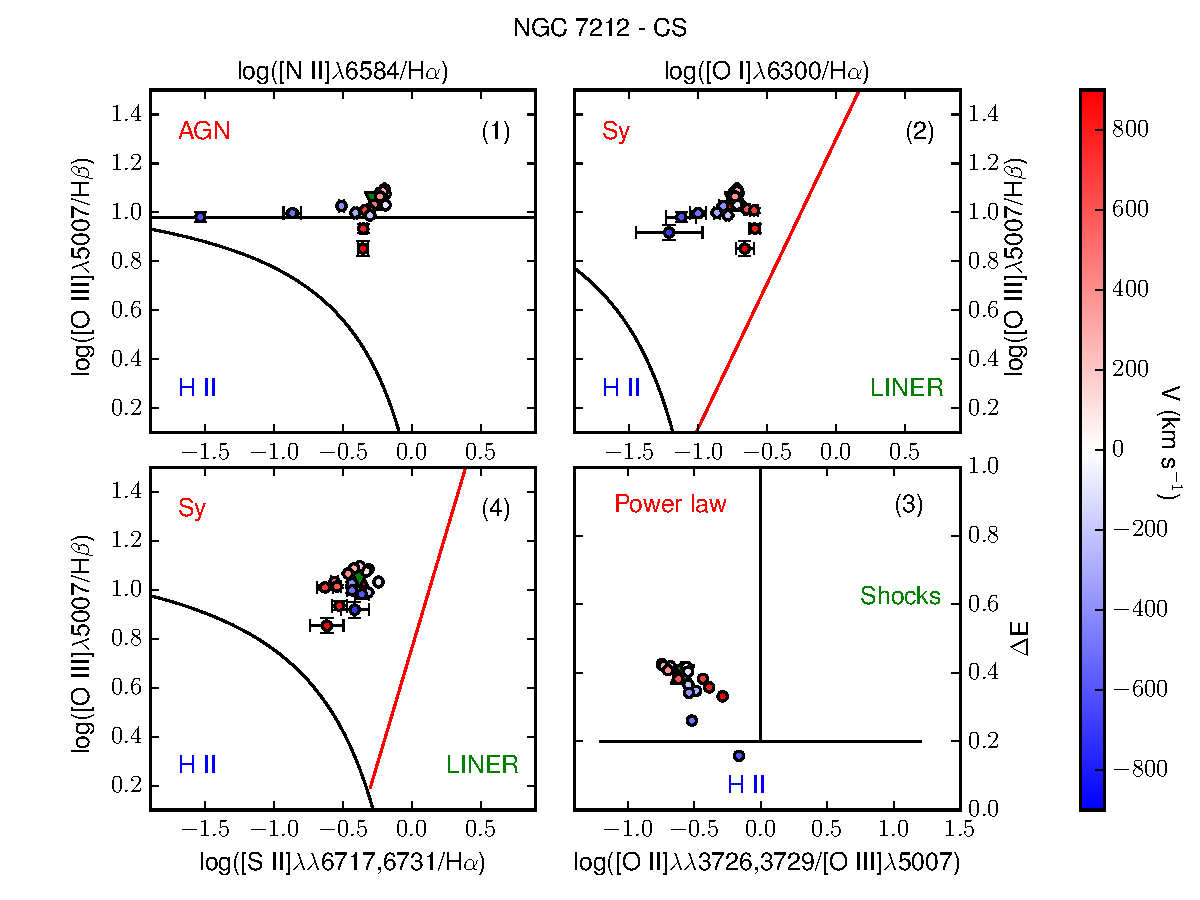
\includegraphics[width=0.43\textwidth]{images/paper1/NGC7212_cs_diag.pdf}} \quad
\subfloat[][]{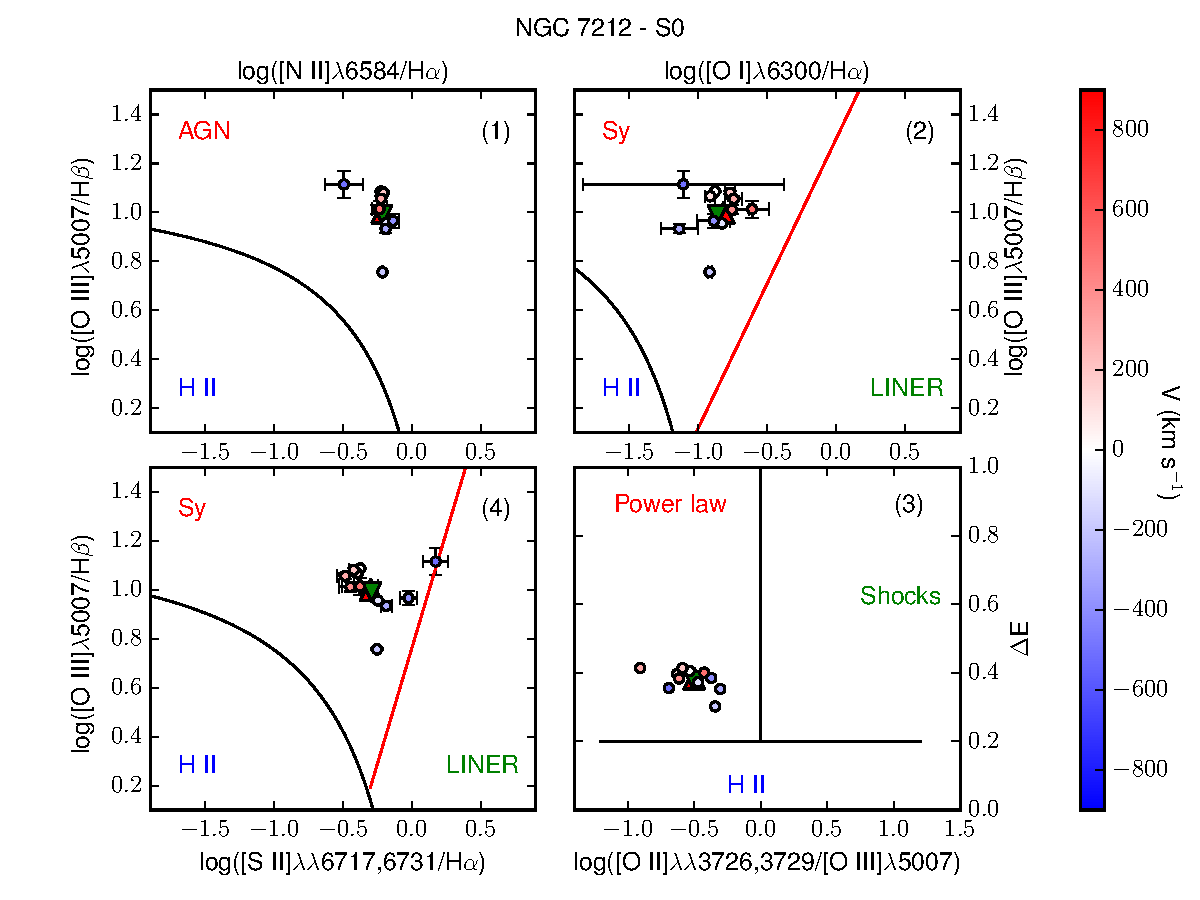
\includegraphics[width=0.43\textwidth]{images/paper1/NGC7212_s0_diag.pdf}}\\
\subfloat[][]{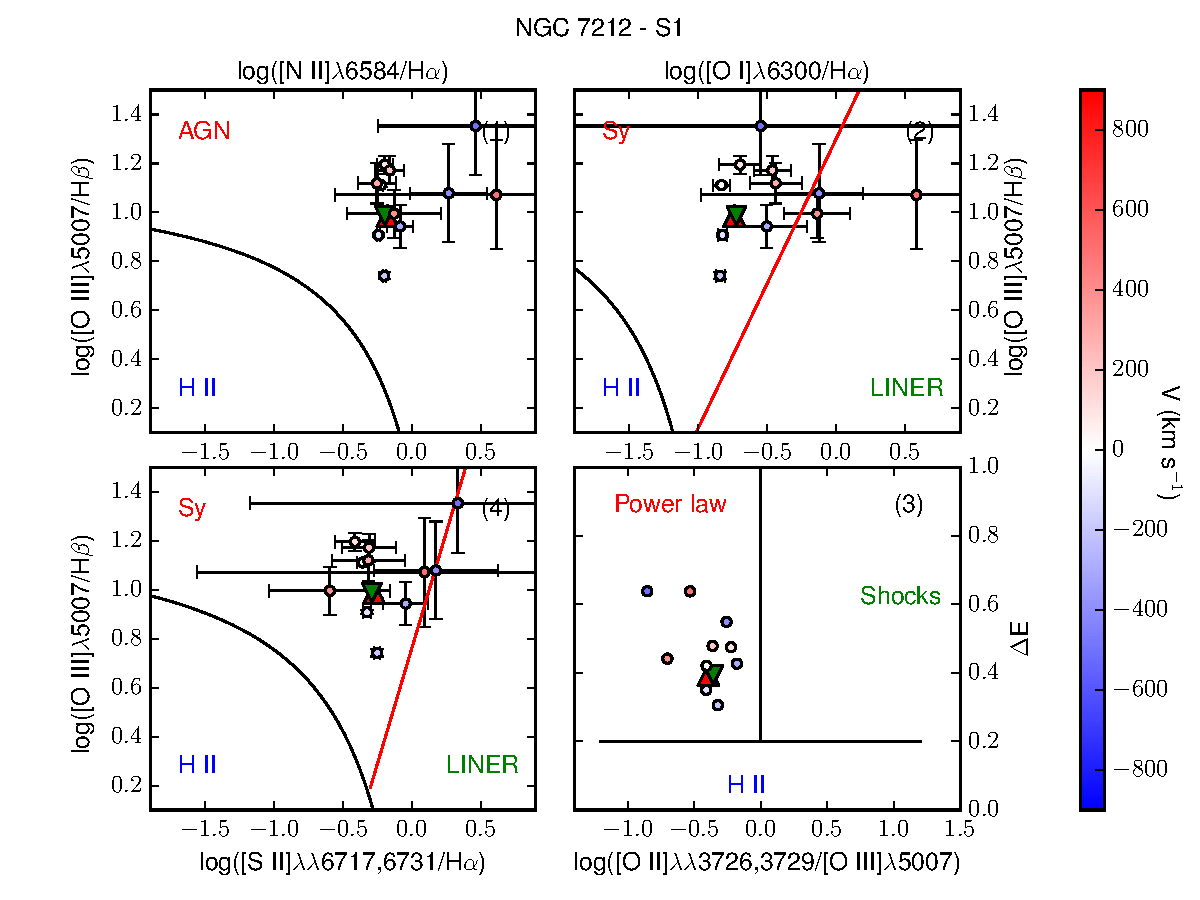
\includegraphics[width=0.43\textwidth]{images/paper1/NGC7212_s1_diag.pdf}}\\
\caption[]{Diagnostic diagrams of the (a) CS, (b) S0 and (c) S1 regions of NGC\,7212. In each plot we show, from the top left panel clockwise: (1) $\log([\ion{O}{III}] \Hb)$ vs $\log([\ion{N}{II}]/ \Ha)$, (2) $\log([\ion{O}{III}]/ \Hb)$ vs $\log([\ion{O}{I}]/ \Ha)$, (3) $\Delta E$ vs $\log([\ion{O}{II}]/[\ion{O}{III}])$, (4) $\log([\ion{O}{III}]/ \Hb)$ vs $\log([\ion{S}{II}]/ \Ha)$ \citep{Baldwin81, Veilleux87}. The colorbar shows the velocity of each bin. The black curves in (1), (2), (4) divide power-law ionized regions (top) and HII regions (bottom). The red lines divide Seyfert-like regions (left) and LINER-like regions (right) \citep{Kewley06}. The black lines in (3) divide HII regions (bottom), power-law ionized region (left) and shock ionized regions (right) \citep{Baldwin81}. }
\label{fig:diag_s1N}
\end{figure*}

\end{document}